\documentclass[sigconf]{acmart}
%% NOTE that a single column version may be required for 
%% submission and peer review. This can be done by changing
%% the \doucmentclass[...]{acmart} in this template to 
%% \documentclass[manuscript,screen]{acmart}
%% 
%% To ensure 100% compatibility, please check the white list of
%% approved LaTeX packages to be used with the Master Article Template at
%% https://www.acm.org/publications/taps/whitelist-of-latex-packages 
%% before creating your document. The white list page provides 
%% information on how to submit additional LaTeX packages for 
%% review and adoption.
%% Fonts used in the template cannot be substituted; margin 
%% adjustments are not allowed.
%%
%%
%% \BibTeX command to typeset BibTeX logo in the docs
\AtBeginDocument{%
  \providecommand\BibTeX{{%
    \normalfont B\kern-0.5em{\scshape i\kern-0.25em b}\kern-0.8em\TeX}}}

%% Rights management information.  This information is sent to you
%% when you complete the rights form.  These commands have SAMPLE
%% values in them; it is your responsibility as an author to replace
%% the commands and values with those provided to you when you
%% complete the rights form.
\setcopyright{acmcopyright}
\copyrightyear{2022}
\acmYear{2022}

%% These commands are for a PROCEEDINGS abstract or paper.
\acmConference[SIGMOD '22] {Proceedings of the 2022 International Conference on Management of Data}{June 12--17, 2022}{Philadelphia, PA, USA.}
\acmBooktitle{Proceedings of the 2022 International Conference on Management of Data (SIGMOD '22), June 12--17, 2022, Philadelphia, PA, USA}
\acmPrice{15.00}
\acmISBN{978-1-4503-9249-5/22/06}
\acmDOI{10.1145/3514221.3517866}
% Authors, replace the X's with your assigned DOI string during the rightsreview eform process.

\settopmatter{printacmref=true}

%%
%% Submission ID.
%% Use this when submitting an article to a sponsored event. You'll
%% receive a unique submission ID from the organizers
%% of the event, and this ID should be used as the parameter to this command.
%%\acmSubmissionID{123-A56-BU3}


%% Put all additions, packages, and customizations in this file


\usepackage{bm} % For bold math in titles
\usepackage{bbm} % For indicator function in appendix \mathbbm{1}
\usepackage{mathtools}  % amsmath with extensions
\let\Bbbk\relax % needed for amssymb as it clashes with something else
\usepackage{amssymb} % needed for traingleq, I guess you can remove if not using
\newtheorem{theorem}{Theorem}
\newtheorem{lemma}[theorem]{Lemma}
\usepackage{algorithm}
\usepackage[noend]{algpseudocode}


\usepackage{xcolor}
\usepackage{listings}
\usepackage{xpatch}
\usepackage{realboxes}

\usepackage{suffix} % provides the \WithSuffix command used to create betterparagraph*
\newcommand{\betterparagraph}[1]{\vspace{2pt} \noindent \textbf{#1:~}}
\WithSuffix\newcommand\betterparagraph*[1]{\betterparagraph{#1}}


% Defines custom \Initialization ... \EndInitialization block
\algdef{SE}[VARIABLES]{Initialization}{EndInitialization}
{\algorithmicinitialization}
{\algorithmicend\ \algorithmicinitialization}
\algnewcommand{\algorithmicinitialization}{\textbf{initialization:}}
\let\oldReturn\Return
\renewcommand{\Return}{\State\oldReturn}

% Tells algorithmicx not to print an empty line if `noend' is set 
\makeatletter
\ifthenelse{\equal{\ALG@noend}{t}}%
{\algtext*{EndInitialization}}
{}%
\makeatother

\algrenewcommand\algorithmicindent{1.0em}

\usepackage{pgf,tikz,pgfplots}
\pgfplotsset{compat=1.14}
\usepackage{mathrsfs}
\usetikzlibrary{arrows}
\usetikzlibrary{math}

%% Externalize tikz
%% Must be in main file for overleaf
%\usetikzlibrary{external}
%\tikzexternalize[prefix=tikzexternalize/]
%\tikzset{external/only named=true}


\usepackage{subcaption}
% Make subfigures look like "3(a)" not "3a"
\captionsetup[subfigure]{labelformat=simple}
\renewcommand\thesubfigure{(\alph{subfigure})}

% for inline lists
\usepackage[inline]{enumitem} 

\DeclarePairedDelimiter\abs{\lvert}{\rvert}%
\DeclarePairedDelimiter\norm{\lVert}{\rVert}%
\DeclareMathOperator{\sign}{sgn}

% Swap the definition of \abs* and \norm*, so that \abs
% and \norm resizes the size of the brackets, and the 
% starred version does not.
\makeatletter
\let\oldabs\abs
\def\abs{\@ifstar{\oldabs}{\oldabs*}}
%
\let\oldnorm\norm
\def\norm{\@ifstar{\oldnorm}{\oldnorm*}}
\makeatother


\lstset{
  language=Python,
  tabsize=4,
  basicstyle=\ttfamily,
  columns=fullflexible,
  keepspaces,
  backgroundcolor=\color{black!10},
  frame=single,
  framerule=0pt,
  xleftmargin=3pt,
}


%% make sure \lstinline has the same bacgrkound
%% https://tex.stackexchange.com/a/357339
\makeatletter
\xpretocmd\lstinline{\setlength{\fboxsep}{1pt}\Colorbox{black!10}\bgroup\appto\lst@DeInit{\egroup}}{}{}
\makeatother

% Curved letters for mathematical formulas
\newcommand{\FA}{\mathcal{A}}
\newcommand{\FR}{\mathcal{R}}
\newcommand{\FB}{\mathcal{B}}
\newcommand{\FD}{\mathcal{D}}
\newcommand{\FH}{\mathcal{H}}
\newcommand{\FS}{\mathcal{S}}
\newcommand{\FU}{\mathcal{U}}



%%
%% end of the preamble, start of the body of the document source.
\begin{document}
\fancyhead{}

%%
%% The "title" command has an optional parameter,
%% allowing the author to define a "short title" to be used in page headers.
\title{AutoMon: Automatic Distributed Monitoring for Arbitrary Multivariate Functions}


%%
%% The "author" command and its associated commands are used to define
%% the authors and their affiliations.
\author{Hadar Sivan}
\affiliation{%
  \institution{Technion -- Israel Institute of Technology}
  \city{Haifa}
  \country{Israel}
}
\email{hadarsivan@cs.technion.ac.il}

\author{Moshe Gabel}
\affiliation{%
  \institution{University of Toronto}
  \city{Toronto}
  \country{Canada}
}
\email{mgabel@cs.toronto.edu}

\author{Assaf Schuster}
\affiliation{%
  \institution{Technion -- Israel Institute of Technology}
  \city{Haifa}
  \country{Israel}
}
\email{assaf@cs.technion.ac.il}

%%
%% By default, the full list of authors will be used in the page
%% headers. Often, this list is too long, and will overlap
%% other information printed in the page headers. This command allows
%% the author to define a more concise list
%% of authors' names for this purpose.
%\renewcommand{\shortauthors}{Trovato and Tobin, et al.}

%%
%% The abstract is a short summary of the work to be presented in the
%% article.
\begin{abstract}

Approaches for evaluating functions over distributed data streams are increasingly important as data sources become more geographically distributed. 
However, existing methodologies are limited to small classes of functions, requiring non-trivial effort and substantial mathematical sophistication to tailor them to new functions.

In this work we present AutoMon, the first general solution to this problem. 
AutoMon enables automatic, communication-efficient distributed monitoring of arbitrary functions. 
Given source code that computes a function from centralized data, the AutoMon algorithm approximates the function over the aggregate of distributed data streams, without centralizing data updates.

Our evaluation shows that AutoMon sends the same number or fewer messages as state-of-the-art techniques when monitoring specific functions for which a distributed, hand-crafted solution is known. 
AutoMon, however, is a lot more powerful. 
It automatically generates a communication-efficient distributed monitoring solution for arbitrary functions, e.g., monitoring deep neural networks inference tasks for which no non-trivial solution is known.

\end{abstract}


%%
%% The code below is generated by the tool at http://dl.acm.org/ccs.cfm.
%% Please copy and paste the code instead of the example below.
%%
\begin{CCSXML}
<ccs2012>
   <concept>
       <concept_id>10003752.10003809.10010172</concept_id>
       <concept_desc>Theory of computation~Distributed algorithms</concept_desc>
       <concept_significance>500</concept_significance>
       </concept>
   <concept>
       <concept_id>10003752.10003809.10010055</concept_id>
       <concept_desc>Theory of computation~Streaming, sublinear and near linear time algorithms</concept_desc>
       <concept_significance>300</concept_significance>
       </concept>
   <concept>
       <concept_id>10002951.10002952.10002953.10010820.10003208</concept_id>
       <concept_desc>Information systems~Data streams</concept_desc>
       <concept_significance>300</concept_significance>
       </concept>
   <concept>
       <concept_id>10003752.10003753.10003760</concept_id>
       <concept_desc>Theory of computation~Streaming models</concept_desc>
       <concept_significance>300</concept_significance>
       </concept>
   <concept>
       <concept_id>10002951.10002952.10003190.10010842</concept_id>
       <concept_desc>Information systems~Stream management</concept_desc>
       <concept_significance>300</concept_significance>
       </concept>
 </ccs2012>
\end{CCSXML}

\ccsdesc[500]{Theory of computation~Distributed algorithms}
\ccsdesc[300]{Theory of computation~Streaming, sublinear and near linear time algorithms}
\ccsdesc[300]{Information systems~Data streams}
\ccsdesc[300]{Theory of computation~Streaming models}
\ccsdesc[300]{Information systems~Stream management}

%%
%% Keywords. The author(s) should pick words that accurately describe
%% the work being presented. Separate the keywords with commas.
\keywords{distributed streams; functional monitoring; approximation}

%%
%% This command processes the author and affiliation and title
%% information and builds the first part of the formatted document.
\maketitle


\section{Introduction} \label{sec:introduction}

Consider the problem of determining whether a network is currently under attack using the aggregate of local statistics from multiple routers~\cite{2015_Bohatei}.
State-of-the-art approaches use machine learning models trained to detect attacks or find outliers given network metrics~\cite{8066291, 10.1016/j.cose.2014.05.011}.
%
For example, we might detect attacks by continuously evaluating the output of a trained neural network:
\[
    f_{nn}(\bar{x}) = W_3 \cdot \tanh \left( W_2 \cdot \tanh \left( W_1 \cdot \bar{x}  + b_1  \right) + b_2  \right) + b_3 \text{~,}
\]
where the input vector $\bar{x}=\frac{1}{k}\sum_{i=1}^{k} x^i$ is the average of $k$ \emph{dynamic} router metric vectors $x^i \in \mathbb{R}^d$ that change over time,
the matrices $W_i$ and vectors $b_i$ are the weights of the neural network, and $\tanh$ is applied element-wise.
In a centralized setting, computing $f_{nn}$ is a straightforward task for the average software developer:
\begin{lstlisting}
from numpy import tanh
def f_nn(x, W1, b1, W2, b2, W3, b3):
   return W3 @ tanh(W2 @ tanh(W1 @ x + b1) + b2) + b3
\end{lstlisting}
When the vectors $x^i$ change, we can simply recompute $f_{nn}(\bar{x})$ as needed, assuming sufficient computational power.

However, the problem becomes much more difficult once the vectors $x^i$ are distributed, even if we assume sufficient computational power and allow an approximation of $f_{nn}$ rather than computing the exact value.
The root problem is that $f_{nn}$ is highly non-linear, making it difficult to understand how it will be affected by a change in $x^i$.
Although, in theory, we could centralize all data updates, this can be infeasible or undesirable in a geographically-distributed environment since communication incurs power and bandwidth costs at the origin nodes of $x^i$~\cite{kang2017neurosurgeon,anastasi2009energy,Stylianopoulos2018gmsystems}.
Returning to our previous example, continuously sending statistics from the routers may use up too much network bandwidth~\cite{gigascope,gabel:entropy_approximation,giatrakos2012prediction,2019_nitrosketch}.
Yet, only sending periodic updates risks missing or delaying the detection of an attack~\cite{benbasat2018memento,gabel:entropy_approximation}.
Resource-limited data sources in mobile computing and Internet-of-Things have further heightened the need for communication-efficient distributed data stream monitoring~\cite{distributed_data_management,ecmlpkdd2019,ecmlpkdd2020}, since the wide geographical distribution of data sources coupled with resource limitation prohibits centralizing all data updates~\cite{garofalakis2013sketch}.
Other scenarios where complex decisions must be made based on global data include battery-powered wireless sensor networks and edge computing. 
Distributed monitoring in these settings is hotly studied since centralizing data is impractical due to battery limitations and limited links~\cite{anastasi2009energy,10.1145/3093337.3037698,mortazavi2020feather}.

The task of continuously evaluating a multivariate function from an aggregate of several data vectors that change over time is a variant of \emph{distributed functional monitoring} in the \emph{continuous distributed monitoring model}~\cite{woodruff2012,2011_ke_yidistributed_functional_monitoring,cormode2013}.
Any general approach for this task faces two main challenges.
First, given a function $f$, how can we maintain an estimate of $f(\bar{x})$ while avoiding the need to send all data updates of $x^i$? 
Second, how do we make it accessible to an average software developer, who may not have the mathematical skills required to tailor the approach to a specific problem?


Most existing work on general distributed functional monitoring focuses on a single aspect of the problem.
For example, while Geometric Monitoring~\cite{2008_shape_sensitive_gm, lazerson:one_for_all} and Convex Bound~\cite{lazerson:lightweight_monitoring} have been used to compute a wide variety of functions such as variance~\cite{gabel:variance_monitoring}, spectral gap~\cite{yeuda2017graph}, skylines~\cite{papapetrou2014skylines}, and least-squares regression~\cite{gabel:monitoring_least_squares}, applying these approaches for each new function requires in-depth mathematical analysis.
Conversely,  Universal Sketching techniques~\cite{zero_one_frequency_laws} provide multiplicative approximation that are easy to use, but are limited to a subset of monotone functions of item counts (i.e., $\bar{x}$ must be a frequency vector).
Distributed data analysis frameworks~\cite{flink,2018_sonata,mortazavi2020feather,nemo,univmon_2016} 
require no math to use, but can only optimize a limited set of primitives.\footnotemark{} 
Neither approach is suitable for low-communication monitoring of more complex functions such as neural networks (i.e., $f_{nn}$), which can be more accurate in detecting outliers, failures, and network attacks~\cite{10.1016/j.cose.2014.05.011, 10.4108/eai.3-12-2015.2262516}.
\footnotetext{For example, SQL-based approaches are limited to grouping, ordering, count, sum, average, and so on~\cite{wanalytics}, while stream processing frameworks are similarly limited to built-in aggregates, windowing, and maps~\cite{flink}.
Such approaches only express a small part of the space of possible computations~\cite{liu2021sketchy}.}



\betterparagraph{Our Contributions}
We describe AutoMon, short for Automatic Monitoring, an algorithmic building block
that enables automatic distributed functional monitoring for difficult functions for which no hand-crafted solution is known while addressing both of the above challenges.
Given a source code snippet for any function $f$ of the aggregate vector $\bar{x}$ and the desired approximation error, AutoMon \emph{automatically} implements a communication-efficient approximation for $f$ over multiple nodes, each with its own dynamic data vector.
%
In particular, we make the following contributions:
\begin{itemize}[leftmargin=*]
    \item A novel communication-efficient scheme for monitoring arbitrary functions of the global aggregated vector.
    Given a function's source code, we leverage automatic differentiation~\cite{survey_on_automatic_differentiation}, numerical optimization, and the Geometric Monitoring protocol~\cite{lazerson:one_for_all,2021_icde_distance_lemma} to derive local constraints that the nodes can check locally, avoiding communication when changes to local data are too small to violate the approximation bounds.
    
    \item An extensive evaluation on synthetic and real-world datasets, and on a range of different functions, including KL-divergence, inner product, and neural networks (DNN).
    AutoMon provides a superior error-communication tradeoff to existing methods.
    For example, on a DNN approximation task -- for which no efficient distributed approximation is known -- AutoMon 
    reduces number of messages and bandwidth usage by up to two orders of magnitude, compared to centralization.

    \item A prototype open source implementation of AutoMon.
    Our prototype library provides an unobtrusive API designed to facilitate development of stand-alone distributed applications (e.g., neural networks over data streams) and components of data analysis frameworks (e.g., efficient implementation of custom operators in stream processing engines~\cite{flinkuserdefined}).
        
\end{itemize}
    
To the best of our knowledge, AutoMon is the first truly automatic distributed functional-monitoring scheme that supports a wide range of functions defined on arbitrary data, and works directly from the source code of the function to compute without manual mathematical analysis.

AutoMon is available as an open source project on GitHub: \\ \url{https://github.com/hsivan/automon}.
\section{Background} \label{sec:background}

Consider a distributed system with a single coordinator node and $n$ nodes, where each node $i$ holds a \emph{dynamic} local data vector $x^i$ computed from its local data stream; $x^i$ changes arbitrarily over time and nodes only communicate with the coordinator\footnotemark{}~\cite{cormode2013}.
When clear from context, we omit $i$ and use $x$ to denote a local vector.

\footnotetext{
These assumptions are for clarity and are not central to our design.
First, communication need not be direct -- we assume an underlying message passing protocol or distributed control plane.
Similarly, the coordinator holds little state and need not be unique.
AutoMon can be implemented using converge-casting~\cite{bhaduri2008local}, hierarchical violation resolution~\cite{keren2014heterogeneous}, or consensus protocols~\cite{zooKeeper,DPaxos}. %; these are outside the scope of our work.
}

Let $f$ be an arbitrary real multivariate function $f :\mathbb{R}^d \to \mathbb{R}$ of the average vector of local data $\bar{x} = \frac{1}{n} \sum_{i=1}^{n} x^i$.
Given $f$ expressed as code in a high-level language (e.g., Python or C++) and an approximation error bound $\epsilon$, we wish to maintain an $\epsilon$-approximation of $f(\bar{x})$, and do so with minimal communication.
%
This is a variation of the \emph{distributed functional monitoring} task~\cite{woodruff2012}.\footnotemark{}
The difference is that we aim to support arbitrary functions expressed as programs.

\footnotetext{Though not immediately obvious, a huge variety of computations can be expressed as $f(\bar{x}$) by augmenting the local vectors $x^i$~\cite{garofalakis2013sketch, papapetrou2014skylines, lazerson:lightweight_monitoring, lazerson:one_for_all, gabel:entropy_approximation, gabel:monitoring_least_squares,keren2014heterogeneous}.}


Note that we can use threshold monitoring to obtain such an approximation: given a \emph{reference point} $x_0$, which is the value of $\bar{x}$ at some point in time, we can provide an additive approximation by setting two thresholds, $L$ and $U$, to be $f(x_0) \pm\epsilon$ and require that $L \le f(\bar{x}) \le U$;
to obtain a multiplicative approximation of $f(\bar{x})$ we set $L$ and $U$ to $(1\pm\epsilon)f(x_0)$.
As long as $L \le f(\bar{x}) \le U$, $f(x_0)$ is an $\epsilon$-approximation of $f(\bar{x})$; if not, we update $x_0$, $U$, and $L$.

Our strategy is to automatically compute local constraints on the local data of each node.
These constraints should be: 
\begin{enumerate*}
    \item \emph{correct} -- as long as all local constraints hold, the \emph{global condition} $L \le f(\bar{x}) \le U$ is guaranteed to hold; 
 \item \emph{efficient} -- the number of times the local constraints are violated is minimal, resulting in less communication; and
 \item \emph{automatic} -- can be computed using the source code of $f$, without requiring mathematical insight or developer effort.
\end{enumerate*}

Finding local constraints that are correct, efficient, and automatic is a challenging task, and even more so for an arbitrary function.
We now briefly review the necessary background. We describe our method in \S\ref{sec:method} and its implementation details in \S\ref{sec:implementation}.


\betterparagraph{DC Decomposition}
%
We use a \emph{DC decomposition}~\cite{dc_Decomposition} of $f$ to derive local constraints that provide correctness.
%
DC decomposition is a representation of a function as the difference of two convex or concave functions.
We use the term \emph{convex difference} for the representation of a function as a difference of two convex functions, and the term \emph{concave difference} for the representation of a function as a difference of two concave functions.
Hence, if $\check{g}(x)$ and $\check{h}(x)$ are convex functions such that $f(x) = \check{g}(x) - \check{h}(x)$, we can rewrite the global condition $L \le f(\bar{x}) \le U$ as
$\check{g}(\bar{x}) \le \check{h}(\bar{x}) + U$ and $\check{h}(\bar{x}) \le \check{g}(\bar{x}) - L$.
Similarly, if $\hat{g}(x)$ and $\hat{h}(x)$ are concave functions such that $f(x) = \hat{g}(x) - \hat{h}(x)$, then we can rewrite the global condition as
$\hat{h}(\bar{x}) \ge \hat{g}(\bar{x}) - U$ and $\hat{g}(\bar{x}) \ge \hat{h}(\bar{x}) + L$.

\betterparagraph{Automatic Differentiation}
We use \emph{automatic differentiation} (AD) to find a DC decomposition of a function.
AD is a general method for taking a function specified by a computer program and automatically constructing a procedure to compute the derivatives of that function~\cite{survey_on_automatic_differentiation}.
Unlike symbolic differentiation, which outputs a closed-form symbolic formula for the derivative, AD outputs a computational graph that can be evaluated efficiently at runtime for specific inputs.
This means AD can be applied to standard numeric program code, making it suitable for our purposes.
Upon initialization, AD explicitly constructs the computational graph of the function, and repeatedly applies the chain rule to this graph to compute the function's derivatives of arbitrary order.
This results in a procedure for computing derivatives.



\betterparagraph{Geometric Monitoring Protocol}
%
AutoMon adopts the geometric monitoring (GM) protocol for continuous threshold monitoring in a distributed system, which has been widely adopted by distributed monitoring methods \cite{gabel:entropy_approximation,gabel:monitoring_least_squares,gabel:variance_monitoring}.
\S\ref{sec:method} provides a detailed description of the AutoMon protocol; what follows is a brief summary of the generic GM protocol.

The GM protocol comprises two basic parts: the coordinator algorithm and the node algorithm.
Each node receives local data and updates its dynamic local vector $x$.
A node is responsible for monitoring the local constraints, reporting violation of these constraints to the coordinator, and receiving updated constraints from the coordinator.
The correctness of local constraints guarantees that if all nodes have no reported violation, the global condition is maintained.
%
The coordinator is responsible for resolving violations of the local constraints by distributing updated local constraints to nodes or approximation bounds $L,U$, as needed.
When the coordinator is notified of local violations, it collects the local vectors from the nodes and, if needed, also updates the reference point $x_0$ to the average vector $\bar{x}$ at the time.
After the data centralization, the coordinator computes new local constraints that resolve the violations and synchronizes the nodes with the new constraints.


%% Central concepts in GM
Let $\FD$ denote the domain where $f(x)$ is defined.
GM defines an \emph{admissible region} $\FA$ as the subset of $\FD$, where $L \le f(\bar{x}) \le U$.
Given a local constraint, GM also defines a \emph{safe zone}: the subset of $\FD$ in which the local constraints of a node are satisfied.
If the safe zone is convex and is a subset of the admissible region, the GM protocol guarantees that the approximation bound defined by the thresholds (i.e., the global condition $L \le f(\bar{x}) \le U$) is maintained~\cite{gabel:entropy_approximation,lazerson:one_for_all}.
When the resulting safe zone is not convex, this gives rise to the possibility of \emph{missed violations}.
This occurs when the global condition is not maintained ($\bar{x}$ is outside the admissible region), yet there is no violation in any of the local constraints.


\betterparagraph{Automatically Deriving Local Constraints}
The GM protocol itself is conceptually simple, since much of the ``heavy lifting'' is done by the local constraint required by the protocol.
Indeed, the convexity of the safe zone is a key non-trivial requirement on the local constraint.
Previous work relied on manual analysis and researcher expertise to find local constraint for specific functions~\cite{gabel:entropy_approximation,yeuda2017graph,papapetrou2014skylines,gabel:monitoring_least_squares,gabel:variance_monitoring}.
However, we are faced with the greater challenge of doing so automatically for arbitrary functions expressed as code, without requiring in-depth mathematical analysis of each function.
In the next section, we describe how we overcome this challenge using automatic differentiation and numerical optimization.

\section{Automatic Distributed Monitoring} \label{sec:method}

We aim to provide an automatic method for distributed monitoring of arbitrary functions of the global aggregate $\bar{x}$.
Given a function specified by a computer program, we automatically generate a communication-efficient scheme to monitor this function.

We first describe ADCD (for \emph{Automatic DC Decomposition}), the automatic local constraint technique that lies at the heart of AutoMon.
ADCD uses automatic differentiation and numerical optimization to derive local constraints for arbitrary functions.
We describe two variants of ADCD, one for general functions (\S\ref{sec:adcd_by_extreme_eigenvalue}) and the other for functions with constant Hessian (\S\ref{sec:adcd_by_eigendecomposition}).
ADCD detects the type of the function and uses the best ADCD variant accordingly to provide a DC decomposition, which it then converts to a GM-style local constraint (\S\ref{sub_sec:adcd}) that can be plugged-in to the GM protocol.
%
We also explore how the type of DC decomposition (convex or concave)  affects the quality of the derived constraints, and propose a heuristic for choosing between convex difference and concave difference (\S\ref{sub_sec:convex_vs_concave_difference}). 

We then describe how AutoMon combines ADCD with the GM protocol to do functional monitoring~(\S\ref{sub_sec:basic-protocol}).
%
Additionally, we consider a novel aspect of the problem: the impact of limiting the monitoring to a small part of the domain in a neighborhood around the reference point, using local constraints that are customized to this neighborhood (\S\ref{sub_sec:sub_domain_size}).
%
Finally, we discuss correctness guarantees (\S\ref{sec:correctness_guarantees}) and implementation considerations (\S\ref{sec:implementation}).


\subsection{ADCD by Extreme Eigenvalue (ADCD-X)} \label{sec:adcd_by_extreme_eigenvalue}

The following lemma shows how to obtain a DC decomposition of a twice differential function $f(x)$.
Recall a function $f$ is convex if and only if its Hessian $H$ is positive semidefinite (denoted $H \succeq 0$), i.e., its smallest eigenvalue is non-negative.
Conversely, $f$ is concave if its largest eigenvalue is non-positive, $H \preceq 0$.
The idea behind the lemma is that $f$ can be ``made convex'' by adding another function such that the Hessian is positive semidefinite (PSD).
The added function must be convex and the difference between the altered function and the added function is the required DC decomposition.
The added function construction is based on the extreme eigenvalues of the Hessian of the function.
Note, the lemma is defined over some set $\FS$, which can be the full domain $\FD$ or a subset of it.

\begin{lemma} \label{lemma:adcd_by_extreme_eigenvalue}
Let $f(x)$ be a twice differentiable function with domain $\FD$, and let $\FS \subseteq \FD$ be a subset of the domain. 
Let $\lambda_{\min}$ and $\lambda_{\max}$ be the smallest and largest eigenvalues of the Hessian $H(x)$ of $f(x)$ where $x\in \FS$,
and define $\lambda^{-}_{\min} \coloneqq \min\{0, \lambda_{\min}\}$ and $\lambda^{+}_{\max} \coloneqq \max\{0, \lambda_{\max}\}$.

Then \eqref{eq:lemma1-convex} is a convex difference of $f(x)$ over $\FS$:
\begin{align}
\label{eq:lemma1-convex}
f(x) = \underbrace{f(x) + \frac{1}{2}\abs{\lambda^-_{\min}} \norm{x-x_0}^2 }_{\text{convex }\check{g}(x)} - \underbrace{\frac{1}{2}\abs{\lambda^-_{\min}} \norm{x-x_0}^2}_{\text{convex }\check{h}(x)}
\end{align}
and \eqref{eq:lemma1-concave} is a concave difference of $f(x)$ over $\FS$:
\begin{align}
\label{eq:lemma1-concave}
f(x) = \underbrace{ f(x) - \frac{1}{2}\lambda^{+}_{\max} \norm{x-x_0}^2 }_{\text{concave }\hat{g}(x)} - \underbrace{\frac{-1}{2}\lambda^{+}_{\max} \norm{x-x_0}^2}_{\text{concave }\hat{h}(x)}.
\end{align}
\end{lemma}


The proof of Lemma~\ref{lemma:adcd_by_extreme_eigenvalue} uses the fact that $\lambda^{-}_{\min} \leq \lambda_{\min}$ to show that Hessians of $\check{g}$ and $\check{h}$ are PSD, which implies $\check{g}$ and $\check{h}$ are convex, and similarly show that $\hat{g}$ and $\hat{h}$ are concave.
The full proof is omitted due to space limitation.


Lemma~\ref{lemma:adcd_by_extreme_eigenvalue} shows how to construct a DC decomposition if we are given the extreme eigenvalues.\footnote{An informal version of \eqref{eq:lemma1-convex} appears in~\cite{lazerson:lightweight_monitoring}, where it is used for manual analysis of specific functions rather than automatically for general function.}
Alas, finding the extreme eigenvalues of a general function, with an $x$-dependent Hessian matrix, is a difficult task~\cite{interval_matrix_branch_and_bound}.
The Hessian $H(x)$ is a function of $x$, and therefore its eigenvalues are a function of $x$.
Finding the $x$ in $\FS$ that obtains the minimal or maximal eigenvalue is not trivial.
Therefore, instead of finding the extreme eigenvalues analytically, we use numerical techniques to solve this problem.


\betterparagraph{Using Automatic Differentiation}
Using Lemma~\ref{lemma:adcd_by_extreme_eigenvalue} requires obtaining $H(x)$ and finding $x',x'' \in \FS$ that obtain $\lambda_{\min}$ and $\lambda_{\max}$.
Our key insight here is that we do not need an analytic solution for $\lambda_{\min}$ and $\lambda_{\max}$, nor a symbolic expression of $H(x)$, but rather a way to evaluate $H$ for specific points in $\FS$.
Since we are given an arbitrary $f(x)$ in the form of a short program, AD enables this automatic evaluation of $H$ in any $x \in \FS$.
By evaluating $H$ using AD at multiple points in $\FS$, and computing the extreme eigenvalues of each such Hessian, we can find the global minimum and maximum $\lambda_{\min}$ and $\lambda_{\max}$.
Instead of evaluating $H$ at random points, we define and solve an optimization problem, which is a more robust and efficient method to find these extreme values.

Another advantage of using AD is that it allows us to apply Lemma~\ref{lemma:adcd_by_extreme_eigenvalue} to functions that are not strictly twice-differentiable.
As demonstrated by the DNN with ReLU activation in \S\ref{sec:evaluation}, AD allows us to surpass this limitation as long as the function is continuous.


\betterparagraph{Finding the Eigenvalues}
After having $H(x)$ computed by AD, and the ability to evaluate it at every $x \in \FS$, we can now use it to find the extreme eigenvalues.
For this $H(x)$, we define two functions, $\lambda_{\min} \left( H(x) \right)$ and $\lambda_{\max} \left( H(x) \right)$, which yield the minimal and maximal eigenvalues of the Hessian, respectively, at a given point $x$.
We then use numerical box-constrained optimization methods (e.g., SLSQP and L-BFGS-B) to solve two optimization problems over $\FS$:
\begin{align} \label{eq:numerical_eigenvalues}
\hat{\lambda}_{\min} = \min_{x \in \FS} \lambda_{\min} \left( H(x) \right),\quad
\hat{\lambda}_{\max} = \max_{x \in \FS} \lambda_{\max} \left( H(x) \right).
\end{align}
These optimization problems are not convex, and their complexity is determined by the function $f(x)$ and its Hessian.
Therefore, there is no guarantee that the solution found by the optimization process is the global solution over $\FS$.
The numerical optimization algorithm could converge to a local minimum/maximum, a saddle point, or even not fully converge, as the number of iterations of the algorithm is limited and the problem could be ill-conditioned and require more iterations.
Hence, $\hat{\lambda}_{\min}$ and $\hat{\lambda}_{\max}$ may be different from the true $\lambda_{\min}$ and $\lambda_{\max}$.
We discuss the impact on correctness in \S\ref{sec:correctness_guarantees}.




\subsection{ADCD by Eigendecomposition (ADCD-E)} 
\label{sec:adcd_by_eigendecomposition}


DC decomposition, the representation of a function $f(x)$ as a difference of two convex/concave functions, is not unique.
Lemma~\ref{lemma:adcd_by_extreme_eigenvalue} in the previous section presented a specific DC decomposition of a function, in which the two functions are constructed using the eigenvalues of $f(x)$.
In this section, we present ADCD-E, another DC decomposition for functions with constant Hessian.
We show that this DC decomposition is superior to ADCD-X for this type of function.
The decision whether to use ADCD-E or ADCD-X is done automatically by our algorithms, as it able to automatically identify the type of the function.

The main idea behind ADCD-E is to use eigendecomposition to split the Hessian of $f(x)$ into two matrices: a positive semidefinite (PSD) matrix $H^+$ and a negative semidefinite (NSD) matrix $H^-$.
This can be done because $H$ is a constant matrix.
We obtain a convex difference of $f(x)$ using $H^-$ instead of $\lambda^{-}_{\min}$, and a concave difference using $H^+$ instead of $\lambda^{+}_{\max}$.
As before, we use automatic differentiation tools to obtain $H$, $H^-$, and $H^+$ .


\begin{lemma} \label{lemma:adcd_by_eigendecomposition}
Let $f(x)$ be a twice differentiable function with Hessian $H$ that is not a function of $x$ (i.e., it is a constant).
Let $\lambda_1 \le \lambda_2 \le ... \le \lambda_d$ be the eigenvalues of $H$, and $v_1, v_2, ..., v_d$ the corresponding eigenvectors.
The Hessian matrix $H$ is a real symmetric matrix, and can therefore be decomposed as $H=Q \Lambda Q^T$, where $Q$ is an orthonormal matrix whose columns are the eigenvectors of $H$, and $\Lambda$ is a diagonal matrix whose entries are the eigenvalues of $H$.

Let $\Lambda^-$ be a diagonal matrix whose diagonal is $[\lambda_1,...,\lambda_k, 0, ..., 0]$, and $\Lambda^+$ a diagonal matrix with diagonal $[0, ..., 0, \lambda_k+1,...,\lambda_d]$,
where $\lambda_1,...,\lambda_k$ are the negative eigenvalues and $\lambda_{k+1},...,\lambda_d$ are the non-negative eigenvalues.

Let $H^- \coloneqq Q \Lambda^- Q^T$ be the NSD part of $H$, and $H^+ \coloneqq Q \Lambda^+ Q^T$ be the PSD part.
Then a convex difference of $f(x)$ is:
\begin{align*}
f(x) = \underbrace{f(x)-\frac{1}{2} (x-x_0)^T H^- (x-x_0)}_{\text{convex }\check{g}(x)} - \underbrace{ \frac{-1}{2} (x-x_0)^T H^- (x-x_0)}_{\text{convex }\check{h}(x)},
\end{align*}
and a concave difference of $f(x)$ is:
\begin{align*}
f(x) = \underbrace{f(x)- \frac{1}{2} (x-x_0)^T H^+ (x-x_0)}_{\text{concave }\hat{g}(x)} - \underbrace{\frac{-1}{2} (x-x_0)^T H^+ (x-x_0)}_{\text{concave }\hat{h}(x)}.
\end{align*}
\end{lemma}


\begin{proof}
    Because $\Lambda = \Lambda^- + \Lambda^+$, hence $H = Q \Lambda Q^T = H^- + H^+$.
	The Hessian of $\check{g}(x)$ is $H - H^-$, which equals $H^+$.
	The matrix $H^+ = Q \Lambda^+ Q^T$ is PSD by construction since its eigenvalues are all non-negative from the definition of $\Lambda^+$.
	The Hessian of $\check{h}(x)$ is $-H^-$, which is PSD.
	Hence, $\check{g}(x)$ and $\check{h}(x)$ are convex.
    %	
	The proof of concavity for $\hat{g}(x)$ and $\hat{h}(x)$ is similar.
\end{proof}

ADCD-E can only be applied to functions that have a constant Hessian, such as inner products or quadratic forms.
For such functions, ADCD-E is superior to ADCD-X since the former results in a larger safe zone and therefore fewer local constraint violations.
Intuitively, $\check{g}_{1}$ is ``more convex'' than $\check{g}_{2}$,
where $\check{g}_{1}$ is $\check{g}$ from Lemma~\ref{lemma:adcd_by_extreme_eigenvalue} and $\check{g}_{2}$ is $\check{g}$ from Lemma~\ref{lemma:adcd_by_eigendecomposition}.

More formally, for a function with constant $H$, $H_{\check{g}_{1}} \succeq H_{\check{g}_{2}}$.
The proof follows from $H^- + \abs{\lambda^{-}_{\min}} I \succeq 0$, and therefore:
\begin{equation*}
    H_{\check{g}_{1}} = H + \abs{\lambda^{-}_{\min}} I = H^+ + H^- + \abs{\lambda^{-}_{\min}} I \succeq H^+ = H_{\check{g}_{2}},
\end{equation*}
Further, note that $\check{g}_{1}(x_0) = \check{g}_{2}(x_0)$.
This implies $\check{g}_{1} \ge \check{g}_{2}$ for every $x \in \FD$ (and similarly for $\check{h}$), which means the ADCD-X safe zone is a subset of the ADCD-E safe zone.

In summary, a safe zone violation with ADCD-E implies violation with ADCD-X but a violation with ADCD-X does not necessarily imply one with ADCD-E.
%
We can automatically detect functions with a constant Hessian by looking at the computational graph for $H(x)$ that is derived from the automatic differentiation step.

\begin{figure*}
	\centering
	\subfloat[{Admissible region is $[0.927, 2.214]$.}]{
	\label{sub_fig:sine_admissible_region}
	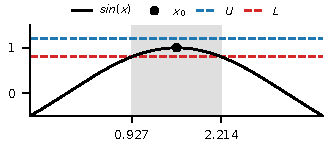
\includegraphics[width=0.32\textwidth]{figures/sine_admissible_region.pdf}
	}
	\subfloat[{Convex difference, safe zone is $[0.928, 2.203]$.}]{
	\label{sub_fig:sine_convex}
	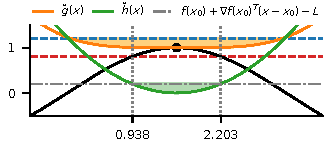
\includegraphics[width=0.32\textwidth]{figures/sine_convex_diff.pdf}
	}
	\subfloat[{Concave difference, safe zone is $[1.121, 2.202]$.}]{
	\label{sub_fig:sine_concave}
	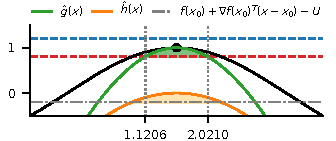
\includegraphics[width=0.32\textwidth]{figures/sine_concave_diff.pdf}
	}
	\caption{
	    ADCD local constraints for $\sin(x)$ at $x_0=\frac{\pi}{2}$.
	    Left: approximation bounds $L$ and $U$ and the resulting admissible region (gray span).
	    Middle: $\check{g},\check{h}$ of the convex difference from Lemma~\ref{lemma:adcd_by_extreme_eigenvalue}.
	    The green area shows the convex set from the upper threshold condition, and the  orange area shows the convex set of the lower threshold condition.
	    The safe zone resulting from their intersection is the area between the vertical dotted lines.
	    Right: same as middle but for $\hat{g}$ and $\hat{h}$ from the concave difference.
	}
	\label{fig:sine}
\end{figure*}




\subsection{From DC Decomposition to Constraints} 
\label{sub_sec:adcd}

After obtaining a DC decomposition of a function, the next step is to derive the ADCD local constraints.
We now show this derivation, and provide a proof that the resulting safe zone is convex, and hence guarantee correctness.

Given a convex difference $f(x) = \check{g}(x) -  \check{h}(x)$, 
we adopt the method of Lazerson et al.~\cite{lazerson:lightweight_monitoring} to derive the ADCD local constraints for $f(x)$ using the tangent plane to $\check{g}(x)$ or $\check{h}(x)$ at $x_0$:
\begin{subequations} \label{eq:convex_condition}
	\begin{align}
	&  \check{g}(x) \le \check{h}(x_0) + \nabla \check{h}(x_0)^T (x - x_0) + U, \\
	& \check{h}(x) \le \check{g}(x_0) + \nabla \check{g}(x_0)^T (x - x_0) - L.
	\end{align}
\end{subequations}
We extend this formulation for the concave difference $f(x) = \hat{g}(x) - \hat{h}(x)$, and obtain the ADCD local constraints for this difference:
\begin{subequations} \label{eq:concave_condition}
	\begin{align}
	& \hat{h}(x) \ge \hat{g}(x_0) + \nabla \hat{g}(x_0)^T (x - x_0) - U, \\
	& \hat{g}(x) \ge \hat{h}(x_0) + \nabla \hat{h}(x_0)^T (x - x_0) + L.
	\end{align}
\end{subequations}
These constraints are convex:
by opening brackets and rearranging the inequality, each inequality can be written as $\psi(x) \le C$, where $\psi$ is a convex function and $C$ is a constant, and the sets that satisfy such inequalities (sublevel sets) are convex~\cite{boyd_convex_2004}.


For the specific convex difference, in Lemma~\ref{lemma:adcd_by_extreme_eigenvalue} and in Lemma~\ref{lemma:adcd_by_eigendecomposition}, the ADCD local constraints \eqref{eq:convex_condition} can be simplified to:
\begin{align*}
\check{g}(x) \le U,\quad
\check{h}(x) \le f(x_0) + \nabla f(x_0)^T (x - x_0) - L.
\end{align*}
For the concave difference the ADCD local constraints \eqref{eq:concave_condition} are:
\begin{align*}
\hat{h}(x) \ge f(x_0) + \nabla f(x_0)^T (x - x_0) - U,\quad
\hat{g}(x) \ge L.
\end{align*}

To get the simplified form of \eqref{eq:convex_condition}, we simply note that for $\check{g},\check{h}$ in both Lemmas, $\check{h}(x_0)=0$ and $\nabla \check{h}(x_0) = 0$ and, $\check{g}(x_0) = \check{f}(x_0)$ and $\nabla \check{g}(x_0) = \nabla \check{f}(x_0)$.
Similarly, we can get the simplified form of \eqref{eq:concave_condition}.




Figure~\ref{fig:sine} shows an example of the ADCD local constraints derived for $\sin(x)$ at point $x_0=\pi/2$ according to Lemma~\ref{lemma:adcd_by_extreme_eigenvalue}.
Figure~\ref{sub_fig:sine_admissible_region} shows the admissible region, while \ref{sub_fig:sine_convex} and \ref{sub_fig:sine_concave} show the ADCD local constraints and the resulting safe zones when using convex and concave difference representations, respectively.
While both safe zones are a subset of the admissible region, they are not equivalent;
We explore this in the next subsection.




\subsection{Convex vs. Concave Difference} \label{sub_sec:convex_vs_concave_difference}

Both ADCD-X and ADCD-E provide two possible representations for a function: as a convex or as a concave difference.
In some cases, a convex difference is more efficient and results in fewer safe zone violations, while in other cases the concave difference is preferable.

Consider again the example in Figure~\ref{fig:sine} showing $\sin(x)$ with the reference point $x_0=\pi/2$.
The convex difference representation in Figure~\ref{sub_fig:sine_convex} results in a wider safe zone than the concave representation in Figure~\ref{sub_fig:sine_concave}.
Since $f$ near $x_0$ is already concave, using the concave difference results in a $\hat{g}(x)$ that is even more concave around $x_0$ than the original function $f(x)$.
However, using the convex difference obtains a convex function $\check{g}(x)$ that is "wider" than the concave function $\hat{g}(x)$, and "wider" functions tend to obtain larger safe zones.
Hence, in this case, the convex difference representation is preferable.

The curvature of $\check{g}$, $\check{h}$, $\hat{g}$, and $\hat{h}$ is determined by the eigenvalues of the Hessians of these functions, and this curvature impacts the performance of the algorithm.
Therefore, we propose the \emph{DC Heuristic} for choosing between the convex difference and concave difference, based on these eigenvalues:
if
\begin{equation*}
    \lambda_{\min} \left( H_{\check{g}}(x_0) \right) + \lambda_{\min} \left( H_{\check{h}}(x_0) \right) \le \abs{ \lambda_{\max} \left( H_{\hat{h}} (x_0) \right) + \lambda_{\max} \left( H_{\hat{g}} (x_0) \right) }
\end{equation*}
use the convex difference, otherwise use the concave difference.

The intuition behind this heuristic is to choose the representation whose two functions are less convex/concave near the reference point $x_0$.
For functions with a constant Hessian, when using ADCD-E, the heuristic condition is equivalent to $\abs{\lambda_{\min}} \le \lambda_{\max}$.

In our preliminary experiments, this heuristic reduced safe zone violations by up to 30\% when compared to using either simply the convex difference or simply the concave difference when monitoring functions such as $\sin(x)$.

\subsection{The Distributed Protocol}
\label{sub_sec:basic-protocol}

We can now describe the protocol for AutoMon coordinator and nodes, which is based on the GM protocol;
the protocol is summarized in Algorithm~\ref{algo:protocol}.
The coordinator first collects local vectors, sets $x_0 = \bar{x}$, and updates the thresholds $U$ and $L$ based on $f(x_0)$ and the desired approximation.
Next, the coordinator uses ADCD to derive correct convex local constraints in a \emph{neighborhood} $\FB$ around $x_0$.
Finally, it distributes these local constraints to all nodes.

\begin{algorithm}
	\caption{AutoMon protocol for coordinator and node.}
	\label{algo:protocol}
	\begin{algorithmic}[1]
		%
		\Procedure{CoordinatorFullSync}{} \label{step:full-sync}
		\State Pull all nodes $x^i$ and update $x_0$: $x_0 \leftarrow \frac{1}{n} \sum_{i=1}^{n} x^i$  \label{step:update-ref-point}
		\State Use $f(x_0)$ to update the thresholds $L$ and $U$
		\State Update the neighborhood $\FB$ from  $x_0$ 
		\State Compute DC decomposition of $f$
		\State Choose between convex difference and concave difference
		\State Derive safe zone based on the chosen DC
		\State Sync all nodes with the safe zone and neighborhood $\FB$
		%
		\EndProcedure

		\Procedure{NodeDataUpdate}{sample from local stream}
		\State Update the local vector $x$ using the new sample
		\If {$x \notin$ $\FB$} Report neighborhood violation and \oldReturn 
		\EndIf \label{step:neighborhood-check}
		\If {$x \notin$ safe zone} Report safe zone violation and \oldReturn
		\EndIf  \label{step:safezone-check}
		\EndProcedure		
		\Procedure{NodeUpdateConstraint}{safe zone, $\FB$}
		\State Update safe zone and the neighborhood $\FB$
		\EndProcedure
	\end{algorithmic}
\end{algorithm}

Let $\FB$ be the neighborhood of size $r$ around the reference point $x_0$: $\FB = \{ x : x \in [x_0-r,x_0+r] \}$.\footnote{In practice, we also restrict the neighborhood $\FB$ to be contained in the domain $\FD$.}
When the neighborhood is restricted, we have two types of violations.
The first type is \emph{safe zone violation}, which is caused when the node's local vector is outside the safe zone.
The second type is \emph{neighborhood violation}, which is caused when the node's local vector is outside the neighborhood of $x_0$.
The coordinator uses either type of ADCD to derive the ADCD local constraints.
For ADCD-X, it applies Lemma~\ref{lemma:adcd_by_extreme_eigenvalue} with $\FS=\FB$.
In this case, the ADCD local constraints are based on eigenvalues that are evaluated inside a specific neighborhood.
Hence, these local constraints are applicable only to this neighborhood:
they maintain correctness as long as all the local vectors are inside $\FB$.
Nodes must therefore first determine that the local vector is inside $\FB$ before checking for a safe zone violation.
Note that when using ADCD-E, the coordinator uses Lemma~\ref{lemma:adcd_by_eigendecomposition}; in this case, the neighborhood is the entire $f$'s domain $\FD$ since the Hessian is constant. 

At initialization, the coordinator first determines whether to use ADCD-X or ADCD-E, depending on the function to approximate $f$ (\S\ref{sec:adcd_by_extreme_eigenvalue} and \S\ref{sec:adcd_by_eigendecomposition}).
If ADCD-E is used, the coordinator evaluates $H^-$ and $H^+$.
If ADCD-X is used, the coordinator uses the designed approximation error bound $\epsilon$ to evaluate the optimal neighborhood size $\hat{r}$ using the tuning algorithm presented in the next section.


The node algorithm is simple: whenever there is an update to the local vector, the node will check if the data remains in the neighborhood $\FB$ and whether the ADCD local constraints still hold.
If not, the node will report a violation to the coordinator.
Otherwise, the node does nothing.
Whenever an updated local constraint arrives from the coordinator, it will use the new constraint.


\betterparagraph{Lazy Sync and Slack}
We incorporate two commonly-used enhancements to the above protocol, which help reduce the number of local violations and allow the coordinator to resolve them without pulling local vectors from all the nodes.
As they are not the focus of this work, we only include necessary detail, and refer the reader to prior work~\cite[Sec.~4.2 and~4.6]{gabel:entropy_approximation} for description and analysis.

With \emph{slack}, nodes add a \emph{slack vector} $s^i$ to the local vector $x^i$ when checking the local constraints (Alg.~\ref{algo:protocol}, lines~\ref{step:neighborhood-check} and~\ref{step:safezone-check});
$s^i$ is set by the coordinator to $x_0 - x^i$ whenever we update $x_0$ (line~\ref{step:update-ref-point}).
%
\emph{Lazy sync} is an incremental approach to resolving safe zone violations.
When a violation is reported to the coordinator, it starts adding nodes one by one to a \emph{balancing set} $\FS$ until either the violation is resolved (in which case it rebalances $s^i$ for the nodes in $\FS$ and monitoring resumes without changing $x_0$), or until $\vert \FS \vert > \frac{n}{2}$ (in which case it falls back to the full sync in line~\ref{step:full-sync}).
We use a least-recently used (LRU) strategy to select nodes to add to $\FS$.
%
We explore the impact of slack and lazy sync in \S\ref{sub_sec:rlv_and_lazy_sync}.

\subsection{Setting the Neighborhood Size} 
\label{sub_sec:sub_domain_size}


ADCD-X requires finding the extreme eigenvalues in a neighborhood $\FB$ of size $r$ around $x_0$.
The choice of neighborhood size $r$ is important since it affects the eventual efficiency of the ADCD local constraints.
An increase in $r$ leads to increase in the search domain for $\lambda_{\min}$ and $\lambda_{\max}$, which can results in more extreme eigenvalues than a smaller $r$ produces, resulting in different DC decomposition.

Interestingly, while prior work observed that different constraints are optimal in different regions of the data space~\cite{lazerson:lightweight_monitoring}, the question of neighborhood size did not come up.
Prior work focused on 
finding analytically-derived constraints designed to be \emph{globally correct}: correct everywhere in $f$'s domain $\FD$.
In contrast, ADCD provides a neighborhood around the reference point, which in turn means the ADCD local constraints need only be correct for data inside the neighborhood $\FB$.
Hence, ADCD constraints are \emph{locally correct}.

\begin{figure}
	\centering
	\subfloat[Smaller neighborhood.]{
	\label{sub_fig:domain_sz_tradeoff_small_domain}
    \quad	
	\scalebox{0.5}{\pagestyle{empty}

\definecolor{ffqqqq}{rgb}{1,0,0}
\definecolor{wrwrwr}{rgb}{0.3803921568627451,0.3803921568627451,0.3803921568627451}
\definecolor{rvwvcq}{rgb}{0.08235294117647059,0.396078431372549,0.7529411764705882}

\begin{tikzpicture}[line cap=round,line join=round,>=triangle 45,x=1cm,y=1cm,yscale=0.8]
\tikzstyle{every node}=[font=\huge]
\begin{scope}
  \clip (-1.2,-0.5) circle (1.441395932235966cm);
  \fill[rvwvcq!20] (-2.4,-1) rectangle (-0.6,1);
\end{scope}
\draw [line width= 1pt,color=wrwrwr] (-1.2,-0.5) circle (1.441395932235966cm);
\draw[line width=1pt,color=black, dashed] (-2.4,-1) rectangle (-0.6,1);

\draw[thick, smooth, color=ffqqqq] plot coordinates
{
	(-3.5,1.3)
	(-3.2,2.2)
	(-0.1,1.8)
	(0.4,0)
	(0.8,-0.6)
	(0.6,-1.2)
	(-0.4,-1.8)
	(-2,-2.4)
	(-2.7,-1.6)
	(-3.7,-0.8)
	(-3.3,0.5)
	(-3.5,1.3)
};

\begin{scriptsize}
\node [fill=black, circle, inner sep=1.5pt, outer sep=1pt, label=above:$x_0$] (x0) at (-1.5,0) {};
\draw [color=black] (-2.513809523809525,1.5) node {$\FB$};
\draw (-1.2,-1.32) node {safe zone};
\draw [color=ffqqqq] (0.15,1.99) node {$\FA$};
\end{scriptsize}
\end{tikzpicture}
}
	\quad
	}
	\qquad
	\subfloat[Larger neighborhood.]{
    \quad	
	\label{sub_fig:domain_sz_tradeoff_large_domain}
	\scalebox{0.5}{\pagestyle{empty}

\definecolor{ffqqqq}{rgb}{1,0,0}
\definecolor{wrwrwr}{rgb}{0.3803921568627451,0.3803921568627451,0.3803921568627451}
\definecolor{rvwvcq}{rgb}{0.08235294117647059,0.396078431372549,0.7529411764705882}

\begin{tikzpicture}[line cap=round,line join=round,>=triangle 45,x=1cm,y=1cm, yscale=0.8]
\tikzstyle{every node}=[font=\huge]
\draw [line width=1pt,color=wrwrwr, fill=rvwvcq!20] (-1.5561710992112803,-0.06440353297281982) circle (0.8580930430876647cm);
\draw[line width=1pt,color=black,dashed] (-4.0,-2.5) rectangle (1.0,2.5);

\draw[thick, smooth, color=ffqqqq] plot coordinates
{
	(-3.5,1.3)
	(-3.2,2.2)
	(-0.1,1.8)
	(0.4,0)
	(0.8,-0.6)
	(0.6,-1.2)
	(-0.4,-1.8)
	(-2,-2.4)
	(-2.7,-1.6)
	(-3.7,-0.8)
	(-3.3,0.5)
	(-3.5,1.3)
};
			
\begin{scriptsize}
\node [fill=black, circle, inner sep=1.5pt, outer sep=1pt, label=above:$x_0$] (x0) at (-1.5,0) {};
\draw [color=black] (-4.35,2.2) node {$\FB$};
\draw (-1.30272727272727273,-1.4) node {safe zone};
\draw [color=ffqqqq] (0.1,2.0) node {$\FA$};
\end{scriptsize}
\end{tikzpicture}
}
    \quad	
	}
	\caption{
		Tradeoff between neighborhood size (dashed rectangle) and the resulting safe zone size (solid circle). 
		The local constraint is their intersection (shaded area).
	}
	\label{fig:domain_sz_tradeoff}
\end{figure}

This presents us with a new opportunity: since ADCD constraints need only be locally correct, they can be more permissive, resulting in fewer safe zone violations.
The challenge lies in balancing the tradeoff between neighborhood and safe zone violations.
%
If the neighborhood $\FB$ is very small (small $r$), the resulting safe zone can be large, but local data easily moves outside the neighborhood, which means more \emph{neighborhood violations (i.e., $x \notin \FB$)}.
If $\FB$ is very large (large $r$) there will be few neighborhood violations, but the resulting safe zone might be needlessly restrictive due to more extreme eigenvalues, resulting in many safe zone violations.
%
Figure~\ref{fig:domain_sz_tradeoff} illustrates this tradeoff.
In Figure~\ref{sub_fig:domain_sz_tradeoff_small_domain} the neighborhood $\FB$ is very small, resulting in a large safe zone but potentially many neighborhood violations.
In Figure~\ref{sub_fig:domain_sz_tradeoff_large_domain} $\FB$ is very large and in fact $\FB$ is a super-set of the admissible region $\FA$ and hence there can be no neighborhood violations.
However, this also results in a much smaller safe zone which could lead to many safe zone violations.




\betterparagraph{Effect of Neighborhood Size $r$}
To explore the impact of the neighborhood size on the number of violations, we used AutoMon to monitor the Rozenbrock function $f(x) = (1 - x_1)^2 + 100 \left(x_2 - x_1^2\right)^2$, where $x_1,x_2$ are sampled from the normal distribution $\mathcal{N}(0, 0.2^2)$.
We used additive approximation with approximation error bound $\epsilon$: $L = f(x_0) - \epsilon, U = f(x_0) + \epsilon$.
For a given approximation error bound $\epsilon$ we monitor the function with different values of $r$, and count the total number of neighborhood and safe-zone violations.

\begin{figure}
	\centering
	{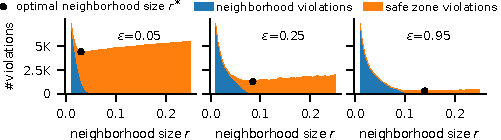
\includegraphics[width=1.0\columnwidth]{figures/impact_of_neighborhood_on_violations_three_error_bounds.pdf}}
	\caption{
	    The effect of neighborhood size $r$ on the number of violations while monitoring Rozenbrock function with four different approximation error bounds.
	}
	\label{fig:impact_of_neighborhood_on_violations_three_error_bounds}
\end{figure}


Figure~\ref{fig:impact_of_neighborhood_on_violations_three_error_bounds} shows the number of violations as a function of neighborhood size for four different approximation error bounds $\epsilon \in \{0.05, 0.25, 0.95\}$.
For a specific $\epsilon$, we observe the tradeoff
between neighborhood violations and safe zone violations.
Additionally, we see that permissive approximation error bounds (larger $\epsilon$) imply larger safe zones, resulting in fewer safe zone violations.
Increasing $\epsilon$ results in slightly more neighborhood violations, which we discuss below.
Lastly, we observe that neighborhood violations decrease when the neighborhood size increases, as expected.



Safe zone and neighborhood violation can hide each other.
Since the nodes check for neighborhood violation before checking the ADCD local constraint, some of the safe zone violations are concealed by neighborhood violations.
However, the opposite also happens.
When $\epsilon$ is small, the resulting small safe zone leads to many safe zone violations. 
When these are resolved, the coordinator updates $x_0$ and the neighborhood $\FB$, meaning that a future neighborhood violations are less likely. 
Therefore smaller $\epsilon$ results in fewer neighborhood violations.

\begin{algorithm}[t]
	\caption{Neighborhood Size Tuning}
	\begin{algorithmic}
		%
		\State $b \gets 1$
		\State \textbf{while} NoNeighborhoodViol(monitor with $r=b$) \textbf{do} $b \gets b / 2$
		\State $lo \gets b$, $hi \gets b$
		\State \textbf{while} AnySafezoneViol(monitor with $r=lo$) \textbf{do} $lo \gets lo / 2$
		\State \textbf{while} AnyNeighborhoodViol(monitor with $r=hi$) \textbf{do} $hi \gets 2\cdot hi$
		\State $R \gets 10$ equally spaced $r$ values in the range $[lo, hi]$
		\Return $\operatorname{argmin}_{r' \in R}$ NumTotalViolations(monitor with $r=r'$)
	\end{algorithmic}
	\label{algo:sub_domain_tuning}
\end{algorithm}



\betterparagraph{Tuning Procedure}
The optimal neighborhood size $r^*$, shown in Figure~\ref{fig:impact_of_neighborhood_on_violations_three_error_bounds} as a dot, is the neighborhood size that obtains the smallest number of violations in total.
The optimal size $r^*$ depends on the function, the data, and the allowed approximation error $\epsilon$.

To avoid the user needing to specify the neighborhood size $r$, AutoMon automatically tunes for the approximated optimal size $\hat{r}$.
This is done by running AutoMon on a small subset of the initial data and counting violations.
Algorithm~\ref{algo:sub_domain_tuning} is the tuning algorithm to find the approximated optimal neighborhood size $\hat{r}$.
It finds a low neighborhood size $r$ for which there are no safe zone violation and a high $r$ with no neighborhood violations, and then returns a neighborhood size in between with fewest total violations.
We evaluate the effectiveness of this tuning procedure in \S\ref{sec:eval-sub-domain-size}.

Since tuning is done on a small subset of the data, later changes in data distribution can mean $\hat{r}$ found by the tuning process becomes too small, causing unnecessary neighborhood violations.
In our experience this is rare, mostly when the error bound is very large.
We mitigate this using a simple heuristic:
whenever the coordinator observes $5 n$ consecutive neighborhood violations with no intervening safe zone violations, it multiplies $\hat{r}$ by 2.
We leave adaptive tuning of $r$ to future work.




\subsection{Assumptions and Correctness Guarantees}
\label{sec:correctness_guarantees}

AutoMon's correctness guarantees are given under three core assumptions.
First, we make the mild assumption that automatic differentiating obtains accurate Hessians.
Second, we assume nodes and coordinator communicate using an underlying messaging fabric which guarantees delivery.
Third, we assume that the rate in which each node receives local data is lower than the maximum time to resolve violations, which depends on the network latency and the time it takes the coordinator to compute local constraints.

Under these assumptions,
AutoMon provides a deterministic correctness guarantee if the representation used to derive the ADCD local constraints is a true DC decomposition in $\FB$, i.e. $\check{g} , \check{h}$ are convex or $\hat{g}, \hat{h}$ are concave in $\FB$.
In this case, the local constraints are convex (\S\ref{sub_sec:adcd}).
This convexity implies that if all local vectors $x^i$ are within AutoMon's safe zone, then any convex combination of $x^i$, including $\bar{x}=\frac{1}{n}\sum x^i$, is inside the safe zone, thus $L \le f(\bar{x}) \le U$.

Therefore, ADCD provides strong correctness guarantee when approximating functions with constant Hessian, as ADCD-E obtains true DC decomposition.
%
In addition, ADCD-X provides correctness guarantee when approximating convex and concave functions.
For any convex function the minimal eigenvalue of $H(x)$ at every $x \in \FD$ is non-negative.
Hence $\hat{\lambda}$ found by the optimization process is non-negative and $\lambda^-_{\min}=0$.
Since $0 \le \lambda^+_{\max}$, the DC Heuristic chooses the convex difference, which is a true DC decomposition as $\lambda^-_{\min}$ is a lower bound for $\lambda_{\min}$.

ADCD-X does not necessarily guarantee correctness for other arbitrary functions since the optimization problem \eqref{eq:numerical_eigenvalues} may converge on a local solution; inaccurate $\lambda^-_{\min}$ and $\lambda^+_{\max}$ values can result in representation that is not a DC decomposition.
%
We mitigate this using a simple sanity check.
Recall that by construction, AutoMon's safe zone defined by the local constraints is included in the admissible region.
Thus, whenever the local vector $x$ is inside the safe zone, nodes also verify that $L \leq f(x) \leq U$ (i.e., $x \in \FA$).
%
In the rare case where this verification fails, the node notifies the coordinator about a violation and indicates that the local constraints are faulty;
the coordinator then initiates a full sync.
%
Our evaluation shows AutoMon provides a good approximation for even highly non-convex functions with discontinuous derivatives
such as neural networks with ReLU activations (\S\ref{sec:evaluation}).


\subsection{Library API} 
\label{sec:implementation}

AutoMon is not a complete distributed data processing system.
Like sketches (\S\ref{sec:related_work}), AutoMon is an algorithmic building block for building such systems (potentially using existing software frameworks~\cite{flink}).
We therefore design AutoMon as an agnostic library that focuses strictly on the monitoring algorithm.
Application details and system-level support for reading data, messaging, deployment, and so on are outside the scope of this library, and are the responsibility of the user.
In particular, the developer must mediate between AutoMon and a messaging fabric of their choice:
the developer uses the library API to produce or consume message contents, which the messaging fabric transfers over the network.\footnotemark{}
\footnotetext{We provide an example of a ZeroMQ~\cite{zeromq} mediation layer in AutoMon's code repo.}


Given a function presented as a numeric program in a high-level language, AutoMon provides the basic API required to perform distributed monitoring of the function.
The user first initializes an AutoMon node, \lstinline[frame=no]{node = AutoMonNode(f, epsilon)}, passing the function to monitor and the required approximation.
Retrieving the current approximated value of the function is simply a matter of calling the \lstinline{node.current_value()} method which returns $f(x_0)$.  
%
The user must notify AutoMon when the local vector $x$ has changed by calling \lstinline{node.update_data(x)}, and send any resulting message (e.g., safe zone violation) to the coordinator;
AutoMon will provide and process the contents of such messages.
Similarly, when a message has been received from the coordinator the user must call \lstinline{node.message_received(msg)}, then send back any reply.

\section{Evaluation} 
\label{sec:evaluation}

We empirically explore AutoMon's performance on several functions of increasing complexity, using both real-world and synthetic data.
In particular, we investigate:
\begin{enumerate}[leftmargin=*]
    \item The tradeoff between communication and approximation error.
    \item Scalability in vector length, runtime, and the number of nodes.
    \item The effectiveness of our neighborhood-size tuning procedure.
    \item The impact of AutoMon's features on the communication cost and accuracy: ADCD local constraints, slack, and lazy sync.
    \item Communication and bandwidth on a real-world WAN.
\end{enumerate}


Our main performance metrics are communication and error.
For communication, we focus on the number of messages sent during an experiment.\footnotemark{} 
Since AutoMon is designed to keep $f(\bar{x})$ between $L$ and $U$, we also measure the maximum error $\vert f(x_0)-f(\bar{x}) \vert$.

\footnotetext{
Though we include bandwidth measurements in \S\ref{sec:distributed-experiment},
we focus on message count for several reasons.
First, we are comparing algorithms, not systems.
The number of messages is a common metric for comparing distributed algorithms because it is independent of any particular network setup and the underlying messaging stack, and because different functions and datasets have different dimensions~\cite{2021_icde_distance_lemma}. 
The size of our payload is fixed and small; given the details above, inferring bandwidth is straightforward.
Second, AutoMon is fully compatible with sketching techniques for reducing message size (see \S\ref{sec:related_work}).
Moreover, there is existing work on reducing the bandwidth of GM-based methods~\cite{2021_icde_distance_lemma,samoladas2019functional}; we leave their implementation for future work.
Lastly, in some settings, the number of messages can be more important than the bandwidth due to the power consumed by turning on the wireless radio~\cite{anastasi2009energy,Stylianopoulos2018gmsystems}.
}

We implemented the prototype in Python.
It uses JAX~\cite{jax2018github} 0.2.1 for automatic differentiation (AD) to compute the Hessian and an L-BFGS-B solver from SciPy~\cite{2020SciPy_NMeth} 1.6.2 to find the extreme eigenvalues.

\subsection{Experimental Setup}

The input for each experiment is the source code for a function $f$ and a dataset comprised of $n$ data streams, one for each node in the system.
The nodes maintain a sliding window over the data stream, and the local vector is defined as the average of the last $W$ samples in the window.
We emphasize that nothing in AutoMon requires a sliding window; it is concerned only with the local vector $x$.

We use discrete event simulation to simulate the distributed network on a single machine.
Most experiments simulate a network of fixed-rate sensors:
in each simulation round, every node reads a data update from its local stream, updates its local vector, and runs the AutoMon node code.
For DNN intrusion detection experiments, only one node reads new data in each round of simulation, using the timestamps encoded in the dataset.
During the experiment, we collect statistics about the messages that are sent between the nodes and the coordinator, the approximation error, missed violations, and so on.
%
In all the experiments, we use AutoMon with Algorithm~\ref{algo:sub_domain_tuning} for neighborhood-size tuning, lazy sync with LRU, and slack.
Unless stated otherwise, we use 10 nodes for the synthetic datasets.

We compare AutoMon with several baseline approaches:

\begin{itemize}[noitemsep, leftmargin=*]
\item \textbf{Centralization:} Every node sends its local vector after every update.
For many distributed functional monitoring tasks, including those that can use sketches, centralization is state-of-the-art since local changes require sending updated sketches~\cite{2021_icde_distance_lemma}.

\item \textbf{Periodic:} Every node sends its local vector once every $P$ simulation rounds (or $P$ time units), where $P$ is a period parameter.
This approach is easy to reason about, but is not adaptive.
It therefore suffers from many missed violations when the period is out of sync with the changes in the data.


\item \textbf{CB:} Convex Bound~\cite{lazerson:lightweight_monitoring} is a state-of-the-art GM-based approach.
For functions with a CB local constraint~\cite{lazerson:lightweight_monitoring}, we include CB in our experiments. 
We run it with lazy sync and slack.

\end{itemize}


\subsection{Functions and Datasets} 
\label{sub_sec:functions_and_datasets}

\begin{figure}
	\centering
	{\label{sub_fig:function_values_and_error_bound_around_it}
	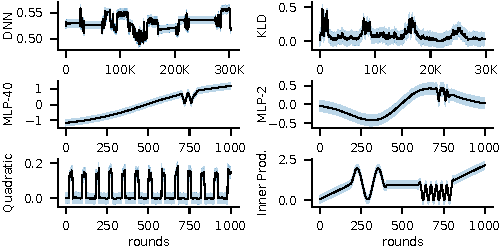
\includegraphics[width=1.0\columnwidth]{figures/function_values_and_error_bound_around_it.pdf}}
	\caption{
	    The functions and datasets used in evaluation.
	    Lines show function value for the default dimension over time;
		shaded area shows approximation bounds $\pm \epsilon$.
	}
	\label{fig:function_value_and_error_bound_around_it}
\end{figure}

We monitor different functions and use different datasets: synthetic for exploring the impact of different parameters on AutoMon and real-world, to evaluate AutoMon's performance over real data.
For synthetic datasets, we used 200 rounds for neighborhood-size tuning data and run the experiment for 1000 rounds.
For real data, the number of rounds is determined by the size of the dataset and we used $\sim 1.5\%$ of the data for tuning.
We now describe the functions that we use and the dataset for each function.
Figure~\ref{fig:function_value_and_error_bound_around_it} shows the value of each function during a run, as well as the additive error bound.
For synthetic datasets, we use the default dimensions, number of nodes, and error bound.

\begin{figure*}
	\centering
	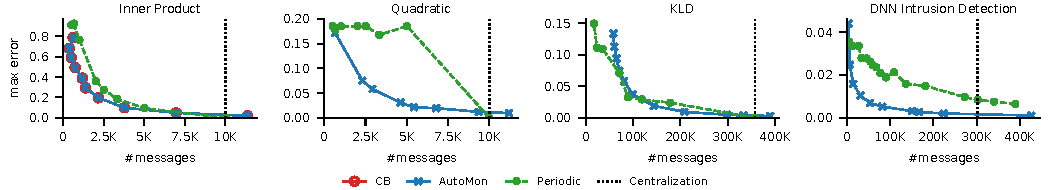
\includegraphics[width=\textwidth]{figures/max_error_vs_communication.pdf}
	\caption{
		Error-communication tradeoff when monitoring different functions with several algorithms;
		lower and to the left is better.
		Each point represents the total number of messages (X axis) and maximum error (Y axis) in one monitoring run, with a specific setting of approximation error bound (or period, for Periodic).
	}
	\label{fig:error_communication_tradeoff}
\end{figure*}

\begin{itemize}[noitemsep, leftmargin=*]


\item \textbf{MLP-}$\bm{d}$\textbf{:}
a neural network with an input layer of dimension $d$, three fully-connected hidden layers with $\tanh$ activation function, and a single output neuron with no special activation (identity function).
The function is therefore:
\begin{align*}
    f(x) =
    W_4 \cdot \varphi \left( W_3 \cdot \varphi \left( W_2 \cdot \varphi \left( W_1 \cdot x  + b_1  \right) + b_2  \right) + b_3 \right) + b_4 \text{~,}
\end{align*}
where $W_i$ and $b_i$ are the respective weights and biases of the hidden layers, and $\varphi$ is the $\tanh$ activation function, applied element-wise.
We trained these weights to evaluate the function  $x_1 \exp \left( - \frac{1}{d-1} \sum_{i=1}^{d}x_i^2 \right)$, and monitor the output of the trained network $f(\bar{x})$.
%
We use a synthetic dataset with $x_1$ sampled from the normal distribution $\mathcal{N}(\mu, 0.1^2)$ with the mean $\mu$ starting at $-2$ and increasing gradually over time.
$x_2, ..., x_d$ are sampled from $\mathcal{N}(2, 0.1^2)$ for half the nodes, and we use $\mathcal{N}(-2, 0.1^2)$ for the remaining nodes.
The data contains some outlier samples:
the mean value of $x_1$ changes to 0 for 20 rounds starting from round 720, and then again from round 760.
The default dimension $d$ in our experiments is 40.






\item \textbf{DNN for Intrusion Detection:}
a deep neural network for intrusion detection, based on the KDDCup-99 dataset~\cite{kddcup99}.
Each sample in the dataset represents a single network connection.
The samples consist of 41 features and are labeled as either normal or an attack.
For this classification task, we used a DNN with 5 fully-connected hidden layers comprising 512, 64, 32, 16, and 8 neurons in each layer, respectively, all using the ReLU activation function.
The output layer contains a single neuron with sigmoid activation.
After using the ``10\% KDD'' dataset to train the network, the trained network achieved 0.933 accuracy, 0.98 precision, and 0.93 recall on the ``Corrected KDD'' test set~\cite{kayacik2005selecting}.

We use the ``Corrected KDD'' test set as the data stream, resulting in a stream of 311029 samples.
%
We divided the data into 9 local streams according to the application-type feature of the data.
For applications that had many samples, we used a round-robin approach for load balancing and divided the samples between multiple nodes: ``ECR\_i'' was divided between 5 nodes and ``Private'' was divided between 2 nodes.
Another single node was responsible for all ``Http'' samples, and the last node was responsible for the other 62 applications.



\item \textbf{KLD:}
The Kullback–Leibler divergence function for discrete probability distributions $P$ and $Q$,
defined on the same probability space $\Omega$: $D_{KL}(P \| Q) = \sum_{\omega \in \Omega} P(\omega) \log \left( P(\omega) / Q(\omega) \right).$

We use a real-world air pollutant dataset~\cite{air_quality_dataset} collected hourly from $n=12$ air-quality monitoring sites in Beijing over 4 years (34,536 data records per site).
For each node (i.e., site), we used the PM10 attribute as $P$ and the PM2.5 attribute as $Q$.
Both attribute values are between 0 and 500, and we divided this range into $d/2$ bins, resulting in a local vector $x=[p,q]$, where $p,q \in \mathbb{R}^{d/2}$ are the local probability vectors for PM10 and PM2.5, respectively;
we use a sliding window of size $W=200$; 
in each round we update $p$ and $q$ with the new measurements.

Since KLD is undefined when $Q$ contains zero entries, we use a common variant which adds a small constant value $\tau$ to the entries of $p$ and $q$ before computing the function
$ f(x)=f([p, q]) = \sum_{i=1}^{d/2} p_i \log \left( p_i / q_i \right)$.
We use $\tau = 1 / \left( n W \right)$, the minimal possible value of the probability vectors in this setting.
Since $f$ is convex, AutoMon's approximation error is guaranteed.

We control the dimension of the function by changing the number of bins $d/2$.
By default, $d=20$.

\item \textbf{Inner Product:}
$f(x)=f([u,v]) = \langle u, v\rangle$, with a synthetic dataset that contains quiet phases as well as rapid changes in the data.
We generated the vectors $u, v \in \mathbb{R}^{d/2}$ such that $f([u,v])$ is a combination of a monotonic increasing function, a sine wave with low and high frequency, and a monotonic constant function.
We control the dimension of the function by changing the dimension of $u$ and $v$.
By default, $d=40$.

\item \textbf{Quadratic Form:}
$f(x) = x^T Q x$, where $Q \in \mathbb{R}^{dxd}$ is a random matrix with entries drawn from a standard normal distribution.
AutoMon uses ADCD-E for this function since its Hessian is constant.
We use synthetic data with each entry of $x \in \mathbb{R}^d$ sampled from the normal distribution $\mathcal{N} (0, 0.1^2)$.
A single ``outlier'' node gets an alternating pattern: 40 samples drawn from $\mathcal{N} (0, 0.1^2)$ followed by 40 samples drawn from $\mathcal{N} (-10, 0.1^2)$.
We use $d=40$.

\end{itemize}



For KLD, the node receives the frequency vector of the samples in the sliding window and the sliding window size is 200 samples.
For the other functions, the node receives the average vector of the samples in the sliding window and the sliding window size is 20 samples.
We start updating the nodes with data only after all the sliding windows of all the nodes are full.




\subsection{Error-Communication Tradeoff} \label{sub_sec:error_communication_tradeoff}
There is an inherent tradeoff between the approximation error and the resulting communication.
A communication-efficient algorithm should use minimal communication and produce a low error.




We compare AutoMon with the baselines for four functions, two with synthetic and two with real-world datasets.
In each run, we monitor the functions using a different approximation error bounds (or period values for Periodic), count the total number of messages and the maximum approximation error, and plot the resulting tradeoff curve.
The best algorithm is the one that achieves the lowest error and communication.
Figure~\ref{fig:error_communication_tradeoff} shows the tradeoff curves of AutoMon and the different baselines.

AutoMon exhibits the best tradeoff overall.
It produces a low error at a fraction of the number of messages needed by Centralization.
It also uses fewer or a similar amount of messages to those required by the non-adaptive Periodic algorithm.

\betterparagraph{Inner Product}
AutoMon automatically achieves identical performance to the carefully tailored CB-based approach of Lazerson et al.~\cite{lazerson:lightweight_monitoring}.
The CB-based algorithm uses the following identity to represent the inner product as a difference between two convex functions: $\langle x,y \rangle = \frac{1}{4}\norm{x+y}^2 - \frac{1}{4}\norm{x-y}^2$.
This form is equivalent to ADCD-E (due to space limitation, the proof is omitted).
While~\cite{lazerson:lightweight_monitoring} provides a CD representation for a specific functions, AutoMon automatically finds such a representation for any function.

\betterparagraph{Quadratic Form}
This function's value can change rapidly, as shown in Figure~\ref{fig:function_value_and_error_bound_around_it}.
The only way to obtain a small approximation error with Periodic is to have a period of 1 (i.e., Centralization); any larger period will result in high approximation errors.
In contrast, AutoMon is adaptive and can provide a smooth, superior, tradeoff between communication and efficiency.

\betterparagraph{KLD}
AutoMon yields a tradeoff that is similar to the Periodic algorithm, but with a smoother, better-controlled tradeoff curve.
Recall however, that the Periodic algorithm is non-adaptive, and the curves in Figure~\ref{fig:error_communication_tradeoff} are derived post-hoc.
Conversely, AutoMon is adaptive and can handle changes in the data distribution.
Moreover, as described above, AutoMon provides a deterministic guarantee for KLD, unlike the Periodic algorithm.

\betterparagraph{DNN}
AutoMon sends fewer messages than Periodic across all $\epsilon$ values.
Unlike the other datasets where local data for all nodes updates every round, the DNN dataset only updates a single node at a time.
This means the function changes gradually, which AutoMon exploits, while the non-adaptive Periodic sends updates from all nodes once per period even when changes are small.
Moreover, since the period parameter now represents a time interval (number of rounds) rather than the number of data samples, Centralization uses fewer messages than Periodic with a period of 1.

\begin{figure}
	\centering
	{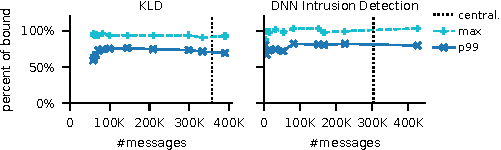
\includegraphics[width=1.0\columnwidth]{figures/percent_error_kld_and_dnn.pdf}}
	\caption{
	    AutoMon communication and error for KLD and DNN.
	    Max (dashed) and 99th percentile (solid) error are shown as percentage of the requested approximation bound.
	    }

	\label{fig:percent_error_kld_and_dnn}
\end{figure}

\betterparagraph{Error Relative to Bound}
Figure~\ref{fig:percent_error_kld_and_dnn} shows AutoMon's relative error with respect to the error bound $\epsilon$ for KLD, where AutoMon guarantees the approximation accuracy (\S\ref{sec:correctness_guarantees}), and for DNN, where there is no such guarantee.
Despite the lack of guarantee, DNN's error profile is similar to KLD:
In practice AutoMon's error is below the approximation bound 99\% of the time for both functions.
Even in the rare cases for DNN when the maximum error is above the bound, it is still very close.

\begin{figure}
	\centering
	\subfloat[Impact of dimension $d$.]{
	    \label{sub_fig:dimension_communication}
	    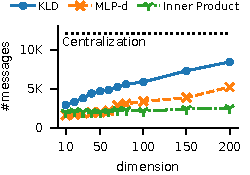
\includegraphics[width=0.47\columnwidth]
	    {figures/dimension_communication.pdf}
	}\hfill
	\subfloat[Impact of number of nodes $n$.]{
	    \label{fig:num_nodes_vs_communication}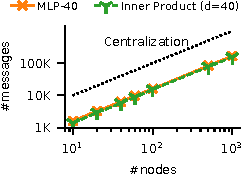
\includegraphics[width=0.47\columnwidth]
	    {figures/num_nodes_vs_communication.pdf}
	}
	\caption{
		Impact of dimension and the number of nodes on AutoMon's communication.
	}	
	\label{fig:dimension_impact}
\end{figure}


\subsection{Scalability: Dimensions, Nodes, Runtime}
\label{sec:scalability}

We use the KLD, Inner Product, and MLP-$d$ functions to study how data dimensionality affects the communication and runtime of AutoMon, as well as its ability to scale with the number of nodes.
For every function, we carry out multiple runs with input dimension $d \in [10,200]$.
As shown below, at high dimensions the bottleneck becomes the numerical optimization in full sync.
To compare the different functions and datasets, we set the number of nodes to $n=12$ and stop each run exactly 1000 rounds after the first sliding window is full,  resulting in a centralized cost of 1000 messages per node.
Runtimes are measured on an Intel i9-7900X at 3.3GHz with 64GB RAM, running Ubuntu 18.04 with MKL 2019 Update 3.


\betterparagraph{Dimensionality}
Prior work has shown that the size of the local vector $x$ can increase the number of messages needed to monitor a function~\cite{gabel:monitoring_least_squares}.
However, for AutoMon, the function itself is also a parameter, and we explore how their combination impacts communication.
Figure~\ref{sub_fig:dimension_communication} shows the total number of messages in each run for different functions and input dimensions.
We observe that AutoMon's scalability is highly dependent on which function is being monitored.
While communication increases with dimension for all functions, this increase is minimal for Inner Product, moderate for MLP-$d$, and more drastic for KLD.
Nevertheless, even for KLD, we observe that AutoMon remains better than centralization for up to 200 dimensions.


\betterparagraph{Number of Nodes}
More nodes means more communication, but this growth is contingent upon the distribution of the data between different nodes.
Figure~\ref{fig:num_nodes_vs_communication} illustrates how the number of messages grows with the number of AutoMon nodes for Inner Product ($d=40$) and MLP-40.
While the number of messages does increase with the number of nodes in the system, we observe that the same happens for Centralization, and that the ratio between Centralization and AutoMon is fixed.
In these synthetic datasets, the data of new nodes is similar to the data of existing nodes.
Therefore, the probability for violation of a single node does not change with the number of nodes, neither does the probability of resolving violations using lazy sync, which explains the fixed ratio.
We therefore conclude that the AutoMon technique does not limit the scalability of the system.
This limitation may emerge from the data itself.


\betterparagraph{Node Runtime}
AutoMon's node runtime should be low since it is targeting environments where the computational power of local data sources is low.
%
We measured the time a node takes to check a single data update, as well as the time it takes the node to complete different tasks during the data update process (figures omitted for lack of space).
The impact of the dimension on the average runtime is negligible, on average 1 millisecond or less for all functions and dimensionality.
The time to verify that the local vector is inside the safe zone is close to the time it takes to simply evaluate the original function on the local vector, ranging from 0.01 to 1 millisecond.
We therefore conclude that AutoMon node is suitable even for computationally limited edge devices.


\betterparagraph{Coordinator Runtime}
While AutoMon's coordinator may not be a resource-constrained edge device, the coordinator's runtime limits the data rate supported by AutoMon because nodes must wait for the coordinator to resolve violations.
This runtime is dominated by the full sync with ADCD-X, which requires solving a numerical optimization problem to find the extreme eigenvalues.
The lazy sync time is orders of magnitude smaller, as it only requires evaluating the local constraints.
%
For KLD and MLP-$d$, which use ADCD-X, the average time for the full sync increases with the dimension, ranging from 0.2 seconds ($d=10$) to 12 seconds ($d=200$).
For Inner Product, the coordinator uses ADCD-E, where eigendecomposition is done only once at initialization; full sync time is below 10 milliseconds for all dimensions.
(Figure omitted for lack of space.)







\subsection{Impact of Neighborhood Size Tuning}
\label{sec:eval-sub-domain-size}

To demonstrate the effectiveness of Algorithm~\ref{algo:sub_domain_tuning},
we show that 
\begin{enumerate*}
\item the $\hat{r}$ found by the algorithm is close to the true optimal neighborhood size $r^*$;
\item $r$ can have a large impact on AutoMon's communication;
\item no single fixed $r$ is optimal across different approximation error bounds $\epsilon$; and
\item the tuning procedure yields comparable performance to using the optimal $r^*$.
\end{enumerate*}


To evaluate Algorithm~\ref{algo:sub_domain_tuning} we used AutoMon with a range of approximation error bounds $\epsilon$ and neighborhood sizes $r$ to monitor the MLP-2 function, as well as the Rozenbrock function, defined as $f(x) = (1 - x_1)^2 + 100 \left(x_2 - x_1^2\right)^2$.
We chose this function because it is especially challenging for gradient-based numerical approaches (e.g., AutoMon or gradient descent), and because its Hessian is non-constant. To generate data, we draw entries $x_1,x_2$ from the normal distribution $\mathcal{N}(0, 0.2^2)$.
%
For each approximation error bound $\epsilon$, we find the optimal neighborhood size $r^*$ that obtains the smallest number of violations, as well as the recommended neighborhood size $\hat{r}$ found by the tuning procedure.
We repeated each experiment $5$ times, sampling a new dataset every run.

On average, the true optimal neighborhood size $r^*$ is close to the neighborhood size found by the tuning procedure $\hat{r}$ (figure omitted due to lack of space), especially given the significant effect of the randomness in the data.
The mean relative error of the tuning algorithm with respect to the optimal value is $8\%$ for Rozenbrock and $20\%$ for MLP-2.
On average, we find that $\hat{r}$ found by Algorithm~\ref{algo:sub_domain_tuning} is within 1.03 standard deviations of the optimal $r^*$ for both functions.
Rozenbrock is highly sensitive to small input changes by design.
Hence, the standard deviation for $\hat{r}$ is large while $r^*$ has a small range (as Figure~\ref{fig:neighborhood_impact_on_communication_error_bound_connection} shows).
Conversely, MLP-2 is less sensitive. 
It has a wider range of optimal $r^*$, while the tuning procedure tends to converge to same $\hat{r}$.


\begin{figure}
	\centering
	{\label{sub_fig:neighborhood_impact_on_communication_error_bound_connection}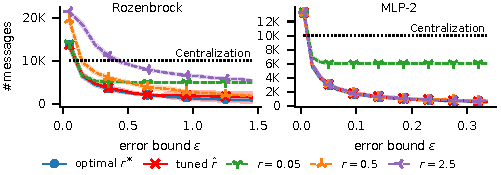
\includegraphics[width=1.0\columnwidth]{figures/neighborhood_impact_on_communication_error_bound_connection.pdf}}
	\caption{
		Mean number of messages for different approximation error bounds $\epsilon$, while using optimal neighborhood size $r^*$, tuned size $\hat{r}$, and fixed $r$ during monitoring.
		The standard deviation is small and barely visible (shaded area).
	}
	\label{fig:neighborhood_impact_on_communication_error_bound_connection}
\end{figure}


To evaluate the impact of $r$ on communication,
we run AutoMon over the sampled datasets, each with its optimal $r^*$ and the tuned $\hat{r}$, as well as three fixed neighborhood sizes $r \in \{0.05, 0.5, 2.5\}$.
Figure~\ref{fig:neighborhood_impact_on_communication_error_bound_connection} shows AutoMon's average communication for each approximation error bound $\epsilon$.
We make three observations.
First, using the wrong $r$ can substantially increase communication.
Second, no single $r$ is best across all $\epsilon$ and functions.
For example, for Rozenbrock the average increase in the number of messages when using $\hat{r}$  instead of $r^*$ is $33\%$, while for the fixed $r$ it grows by more than $100\%$.
For MLP-2, the difference between $r^*$ and $\hat{r}$ is $3.5\%$; however, for the best other fixed $r$ it is more than $7\%$.
The results for MLP-2 also suggest there is a range of neighborhood sizes that work well; however, this range is not known a-priori.
Third, and most crucial, we observe that using the $\hat{r}$ found by the tuning process results in a similar number of messages as using the optimal neighborhood  $r^{*}$.



\subsection{Impact of ADCD, Slack, and Lazy Sync} \label{sub_sec:rlv_and_lazy_sync}

We perform an ablation study to evaluate the contribution of different components of AutoMon.
Could we replace the ADCD local constraints with simply checking the global condition on local data $L \leq f(x) \leq U$, relying on the GM protocol to reduce communication?
As shown below, even for simple functions with only few nodes, this is not the case.


We demonstrate this using the function $f(x) = -x_1^2 + x_2^2$ with four nodes.
We simulate 1000 rounds with the local data for the four nodes initially the same, starting at $(x_1, x_2)=(0,0)$.
As the experiment progresses, local node data slowly drifts in different directions, which is common in distributed setting. Specifically, the local vectors move towards $(1,0)$, $(-1,0)$, $(1,1)$ and $(1,-1)$).
For two nodes, we also add outliers between rounds 650 and 700.


\begin{figure}
	\centering
	\subfloat[$f(x)=-x_1^2+x_2^2$.]{
	    \label{sub_fig:monitoring_stats_quadratic_inverse}
	    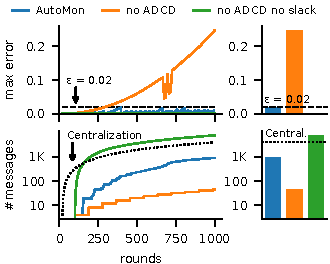
\includegraphics[width=0.65\columnwidth]{figures/monitoring_stats_quadratic_inverse.pdf}
	}
	\subfloat[MLP-2.]{
	    \label{sub_fig:monitoring_stats_barchart_mlp_2}
	    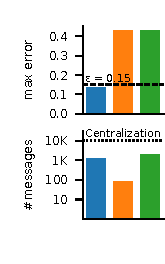
\includegraphics[width=0.32\columnwidth]{figures/monitoring_stats_barchart_mlp_2.pdf}
	}	
	\caption{
	    Impact of AutoMon features on approximation error (top) and cumulative communication (bottom) when monitoring $f(x)=-x_1^2+x_2^2$ (left) and MLP-2 (right); lower is better.
		ADCD and slack are both needed to achieve low error and low communication.
	}
	\label{fig:monitoring_stats}
\end{figure}


Figure~\ref{sub_fig:monitoring_stats_quadratic_inverse} shows the approximation error (top) and cumulative messages (bottom) of each algorithm over time. 
AutoMon maintains the desired approximation error using minimal communication, since the ADCD local constraints for $f$ are both correct and efficient.
Without ADCD, however, the monitoring suffers from missed violations: locally for every node $i$, $L \leq f(x^i) \leq U$, yet globally $L > f(\bar{x})$ or $f(\bar{x}) > U$.
This happens because lazy sync manages to balance the slack of different nodes, preventing the global sync from recomputing the reference point $x_0$.
The end result is unbounded and ever-increasing error, albeit with little communication.
We further removed slack and lazy sync, which gave us a basic GM protocol: similar to Algorithm~\ref{algo:protocol} but without ADCD.
This results in a low approximation error due to many full sync operations, but at the cost of more communication than would be used by a centralization approach (which would result in no error).

We repeated the experiment with the more complex MLP-2 function and present the results in Figure~\ref{sub_fig:monitoring_stats_barchart_mlp_2}.
Without ADCD, the approximation error grows to over twice the size of the bound.
Unlike before, removing the slack and lazy sync mechanism does not help since for MLP-2 it is even more likely that locally $L \leq f(x^i) \leq U$ while globally $L > f(\bar{x})$ or $f(\bar{x}) > U$.
In contrast, AutoMon maintains the desired approximation with low communication by synchronizing as needed.





\subsection{Validation on Real-World Deployment}
\label{sec:distributed-experiment}

Simulations let us compare algorithms while controlling important variables (such as $n$, $d$) in isolation from confounders (e.g., choice of network stack).
%
We now verify our simulation in Section~\ref{sub_sec:error_communication_tradeoff} through a series of geo-distributed experiments.
We conducted each run in our experiments on two Amazon ECS clusters~\cite{amazonecs}: one is located in us-west-2 region and is comprised of a single coordinator using 16 vCPUs and 32GB of memory on an Intel Xeon CPU at 3.4--3.9 GHz;
the other is located in us-east-2 and includes all nodes, each with 1 vCPU and 4GB of memory on an Intel Xeon CPU at 2.2--2.5GHz;
the average RTT was 56ms.
For messaging, we used ZeroMQ~\cite{zeromq}.
We set the time between data updates to 5 seconds for DNN and to 1 second for the other datasets.
We count the total bytes in the payload of AutoMon's messages, and use Nethogs~\cite{nethogs} to monitor the traffic volume of the coordinator process, which includes both payload and overheads such as ZeroMQ and packet headers.

\begin{figure}
	\centering
	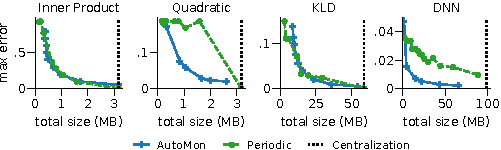
\includegraphics[width=1.0\columnwidth]{figures/max_error_vs_transfer_volume.pdf} 
	
	\vspace{3mm}
	
	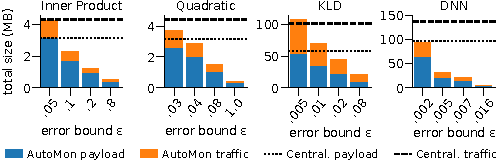
\includegraphics[width=1.0\columnwidth]{figures/communication_automon_vs_network.pdf}
	\caption{
	    Bandwidth usage in distributed experiments over public WAN.
	    Top: error-bandwidth tradeoff, with
	    X axis showing total size of message payload for each monitoring approach.
	    Bottom: AutoMon's total message payload size and measured 
	    network traffic for a range of $\epsilon$ values from the distributed experiments in Figure~\ref{fig:max_error_vs_transfer_volume}.
	    Horizontal lines depict centralization payload size and network traffic.
	}
	\label{fig:max_error_vs_transfer_volume}
	\label{fig:communication_automon_vs_network}
\end{figure}

\betterparagraph{Number of Messages}
Real-world communication matches our simulation, with a median difference of 0\% for the DNN function, less than 5.3\% for inner product and KLD, and 16.6\% for Quadratic (figure omitted).
Slight timing differences when nodes update their local data result in a small number of additional messages, as the coordinator requests the local vectors for nodes after they had already reported a local violation.

\betterparagraph{Error-Bandwidth Tradeoff}
The top of Figure~\ref{fig:max_error_vs_transfer_volume} shows the error as a function of total payload size.
The error-bandwidth tradeoff generally agrees with the error-communication tradeoff in Figure~\ref{fig:error_communication_tradeoff}.
The relative ranking of methods is also the same:
AutoMon's total payload size is lower than that of Periodic whenever AutoMon uses less messages than Periodic.

\betterparagraph{Network Traffic Consumed}
The bottom of Figure~\ref{fig:communication_automon_vs_network} shows AutoMon's total payload size (blue) and actual network usage (orange) for a range of $\epsilon$ values.
The dotted line is Centralization's payload size and the dashed line is its network traffic.
In most cases, except in the extreme cases for a very small $\epsilon$ value, AutoMon's usage is less than Centralization's payload.
It reduces data transfer volumes by up to 98\%, depending on the requested error bound $\epsilon$, and by 65\% on average across all tested functions and error bounds.

\section{Related Work} \label{sec:related_work}


We divide related work on distributed monitoring into five areas.

\betterparagraph{Sketches}
Sketches are comprised of a sketching procedure to reduce the data size, and an appropriate query function that estimates a statistic using the sketch~\cite{2007_rusu_statistical_analysis_of_sketch_estimators}.
They substantially reduce the size of messages required to monitor a function, while offering 
(usually probabilistic) approximation guarantees.
Unlike AutoMon, sketches are generally tailored for specific functions and queries; (e.g., PCA~\cite{Huang2020jmlr});
creating a sketch for a new function is non-trivial, requiring manual effort and significant mathematical sophistication~\cite{2013_opensketch,univmon_2016, liu2021sketchy}.
%
Notably, AutoMon is compatible with most sketches in the turnstile model, since they are linear or can be made linear~\cite{Li_2014_Turnstile}.
AutoMon can monitor a linear sketch by defining $f$ as the query function and $x$ as the sketched data structure, since $\bar{x} = 1/n \sum x^i$.

\betterparagraph{Generic Sketches}
%
Universal Sketches~\cite{zero_one_frequency_laws} provide a distributed approximation for any function from the \emph{Stream-PolyLog} family using a single universal sketch data structure, while requiring no more sophistication than being able to compute the desired function.
Specifically, if $x$ is a vector of counts (frequencies), and $f(x) = \sum g(x_i)$ where $x_i$ are frequency counts and $g$ is monotonic and bounded from above by $O(x_i^2)$, then given an implementation of $g$ universal sketches provide a multiplicative approximation for $f(x)$ with probabilistic guarantees.

Universal sketches are heavily used in the UnivMon framework for network flow monitoring~\cite{univmon_2016}. Similarly, the AutoMon library is an application-agnostic building block for distributed applications and frameworks.
%
Though similar in spirit, universal sketches and AutoMon have different constraints, guarantees, and performance metrics.
First, they are limited to \emph{Stream-PolyLog} functions defined over frequency vector in the turnstyle stream model.
Conversely, AutoMon supports a much wider class of functions and the data vector $x$ can be defined arbitrarily.
Second, universal sketches focuses on providing strong probabilistic guarantees on accuracy.
While AutoMon does provide strong deterministic accuracy guarantee for functions with constant Hessian and for convex and concave functions, we also show empirically that it is accurate even when no such guarantee is provided.
Finally, sketches can reduce the size of each message (by reducing the size of the sketch), while AutoMon focuses on reducing the number of messages exchanged.


Nitrosketch~\cite{2019_nitrosketch} is a general framework for accelerating the computation time of existing sketches such as universal sketches; it does not address designing those sketches automatically.


\betterparagraph{General Algorithms for Distributed Monitoring}
While many works propose distributed algorithms for monitoring specific functions, they tend to use bespoke protocols; applying such methods (e.g., distributed counting) to new functions (e.g., entropy) often requires non-trivial effort and development of new techniques~\cite{cormode2013}.


Some works focus on providing general approaches for distributed function monitoring.
Geometric Monitoring (GM)~\cite{2008_shape_sensitive_gm,lazerson:one_for_all} is a family of communication-efficient approaches to distributed monitoring that share the same underlying protocol of using convex local constraints to monitor a global threshold condition.
These have been used to approximate diverse functions including variance~\cite{gabel:variance_monitoring}, mutual information~\cite{giatrakos2012prediction}, AMS sketches~\cite{garofalakis2013sketch}, linear regression~\cite{gabel:monitoring_least_squares}, and more~\cite{sharfman_2007, lazerson_2015, giatrakos_2014, friedman_2014, keren_2012}.
%
Convex Bound~\cite{lazerson:lightweight_monitoring} leverages ideas from GM as well as \emph{DC decompositions}~\cite{dc_Decomposition} to monitor several non-convex functions; however, again this approach requires mathematical sophistication and cannot be applied automatically.
Samoladas and Garofalakis~\cite{samoladas2019functional} introduce Functional Geometric Monitoring, which replaces the GM protocol with a distributed counting protocol, greatly reducing the size of messages.
As with other methods, it requires finding local constraints (\emph{safe functions}) for each new monitored function.
More recently, Alfassi et al.~\cite{2021_icde_distance_lemma} proposed a ``drop-in'' replacement of the GM protocol to reduce its bandwidth, while relying on the existing local constraints.

Though general, none of these are automatic; they require in-depth mathematical analysis to develop local constraints for new functions.
Gabel et al.~\cite{gabel:entropy_approximation} show how to apply GM automatically but their approach is limited to convex or concave functions.
Conversely, AutoMon derives its local constraints automatically for arbitrary functions of the global vector, directly from source code.



\betterparagraph{Distributed Dataflow and Query Planning}~
Stream processing engines~\cite{flink,spark} execute distributed computation as a data-flow graph of built-in primitive operators.
Other approaches optimize the aggregation network that runs a given query over distributed data~\cite{2018_sonata,mortazavi2020feather,nemo}.
%
Such techniques require expressing the computation using only a limited set of built-in primitives~\cite{2019_yu_network_telemetry}.
For complex numerical functions such as $f_{nn}$ in \S\ref{sec:introduction} or the DNN in \S\ref{sec:evaluation} they are equivalent to centralization or periodic updates.
AutoMon can complement these approaches by optimizing user-defined operators.

\betterparagraph{Geo-Distributed Data Analytics}~
Systems proposed for analyzing geo-distributed data generally fall into one of the above general approaches~\cite{wanalytics,pixida,mortazavi2020feather,tiwari2019reconfigurable}, or are designed for specific tasks using bespoke techniques that do not readily generalize~\cite{gaia,kang2017neurosurgeon,iridium}.

\section{Discussion} \label{sec:discussion}
AutoMon is an easy-to-use algorithmic building block for automatically approximating arbitrary real multivariate functions over distributed data streams.
Given a source code snippet of an arbitrary function of the global aggregate, AutoMon automatically provides communication-efficient distributed monitoring of the function approximation, without requiring any manual analysis by the user.
Our evaluation on synthetic and real-world datasets shows that AutoMon's error-communication tradeoff is comparable to previous hand-crafted algorithms, while using up to 50 times fewer messages on functions for which such efficient algorithms are not known.


Future work will concentrate on addressing AutoMon's limitations, and on improving its accuracy and performance.

First, AutoMon requires that $f$ be a function of the average vector $\bar{x}$, and does not capture functions such as $\sum_i \sum_j x^i x^j$ used in support vector machines~\cite{steinwart2008support}.
Though many functions can be rewritten in terms of $\bar{x}$~\cite{garofalakis2013sketch, lazerson:lightweight_monitoring, lazerson:one_for_all, gabel:entropy_approximation, papapetrou2014skylines, gabel:monitoring_least_squares}, %although
this is currently done manually.
We plan to explore automatic function rewriting, as well as support for more aggregations (e.g., max, sum of inner products).

Second, for functions not covered by the guarantees in \S\ref{sec:correctness_guarantees} the numerical optimization could yield inaccurate extreme eigenvalues and, therefore, violation of the error bounds.
Bounding the Hessian eigenvalues~\cite{2008_bound_hessian_eigenvalues,interval_matrix_branch_and_bound} can alleviate this issue. 
%
We also intend to study what factors impact AutoMon's performance.
The error-communication tradeoff is determined by both the function as well as the data and window size.
For example, when the extreme eigenvalues are exceptionally large/small, the derived safe zone can be very small leading to many safe zone violations.
Inferring this \emph{a priori} is hard for complex, hard-to-analyze functions -- if we could easily understand their behavior analytically, we would not need AutoMon in the first place.
However, we can use such observations to improve performance by switching on the fly to other monitoring approaches (e.g. Periodic).


Lastly, approximation error can be high if numerical optimization in the coordinator takes too long, which limits incoming data rate (\S\ref{sec:correctness_guarantees}, \S\ref{sec:scalability}).
To scale AutoMon to higher dimensions and data rates, we plan to explore Hessian spectrum approximations~\cite{lanczos_algo},
as well as pre-computing future constraints when the coordinator is idle.


\iffalse
In addition to specifying the {\itshape template style} to be used in
formatting your work, there are a number of {\itshape template parameters}
which modify some part of the applied template style. A complete list
of these parameters can be found in the {\itshape \LaTeX\ User's Guide.}

Frequently-used parameters, or combinations of parameters, include:
\begin{itemize}
\item {\verb|anonymous,review|}: Suitable for a ``double-blind''
  conference submission. Anonymizes the work and includes line
  numbers. Use with the \verb|\acmSubmissionID| command to print the
  submission's unique ID on each page of the work.
\item{\verb|authorversion|}: Produces a version of the work suitable
  for posting by the author.
\item{\verb|screen|}: Produces colored hyperlinks.
\end{itemize}


\section{CCS Concepts and User-Defined Keywords}

Two elements of the ``acmart'' document class provide powerful
taxonomic tools for you to help readers find your work in an online
search.

The ACM Computing Classification System ---
\url{https://www.acm.org/publications/class-2012} --- is a set of
classifiers and concepts that describe the computing
discipline. Authors can select entries from this classification
system, via \url{https://dl.acm.org/ccs/ccs.cfm}, and generate the
commands to be included in the \LaTeX\ source.

User-defined keywords are a comma-separated list of words and phrases
of the authors' choosing, providing a more flexible way of describing
the research being presented.

CCS concepts and user-defined keywords are required for for all
articles over two pages in length, and are optional for one- and
two-page articles (or abstracts).
\fi


%%
%% The acknowledgments section is defined using the "acks" environment
%% (and NOT an unnumbered section). This ensures the proper
%% identification of the section in the article metadata, and the
%% consistent spelling of the heading.
\begin{acks}
The authors thank Ran Ben Basat and the anonymous reviewers for their valuable feedback.
The research leading to these results was supported by the Israel Science Foundation (grant No.191/18).
This research was partially supported by the Technion Hiroshi Fujiwara Cyber Security Research Center, the Israel National Cyber Directorate, and the HPI-Technion Research School.
\end{acks}


%%
%% The next two lines define the bibliography style to be used, and
%% the bibliography file.
\bibliographystyle{ACM-Reference-Format}
\balance
\bibliography{main}


\end{document}
\endinput
%%
%% End of file `sample-sigconf.tex'.
